\chapter{DISTRIBUTED CHANNEL AND POWER ALLOCATION IEEE 802.22 NETWORKS}

\section{Motivation}

Secondary users working with TV white space is promising to cope with the scarcity of spectrum resources~\cite{FCC_2010_sedond_memorandumm}. 
Firstly, more unused TV white frequencies become vacant than ever with the ongoing transition from analog to digital broadcasts. Secondly, the frequencies of TV bands enable broadband access over larger geographic ranges compared to higher frequency bands. Nevertheless, services on TV receivers need to be protected with so called interference margin~\footnotetext[2]{interference margin is the maximal interference caused by secondary users, which doesn't violate TV service.}~\cite{multipleIntf_pimrc11} which should not be exceeded by the accumulated interference caused by all secondary users working on the the channel.

\gls{FCC} and \gls{ECC} have announced rules on the transmission power of secondary users working in TV white space in US and Europe respectively~\cite{FCC_2010_sedond_memorandumm, ecc159}. 
FCC requires a minimum distance between secondary user and TV service area, besides, the transmission power for fixed secondary users is set as $4$ \textup{W}, which is a conservative setting. %If the interference margin of the TV receivers can be fully utilized, the requirement on secondary users' transmission power can be relaxed to some extent. 
FCC believes with these prudent measures, the interference margin can not be exceeded by interference from secondary users.
But it may not be the case when there are multiple secondary equipments transmitting at the same time, which is pointed in~\cite{Jaentti11}.
ECC requires the secondary users to adapt their maximum transmission power according to the distance away from the TV receivers.
%In this manner, secondary systems have to determine their maximum transmission power.

FCC issued a memorandum~\cite{FCC_2010_sedond_memorandumm,FCCdatabasae} in 2010, which removes the mandatory rigid sensing requirements, and prompts the usage of geolocations\footnote{Geolocation means both geographic location and terrain.} of secondary users.
FCC regulates a centralized database, which registers all the secondary users within one certain area.
Secondary users can access the database, and can only use the channels assigned by the database.
% thus greatly facilitates the use of the spectrum with geolocation based channel allocation.
Work~\cite{SenseLess2011} follows this rule to obviate spectrum sensing and only relies on the database of TV incumbents to determine the white space availability for secondary users. 
The authors of~\cite{SenseLess2011} demonstrate the feasibility of predicting the available TV spectrum accurately using sophisticated propagation models (Longley-Rice) and geolocations of secondary users. 
A central database contains the geolocations of all TV stations, then the database calculates the received signal strength index (\gls{RSSI}) levels of TV \gls{UHF} signals on all secondary users and accordingly determines the available TV spectrum for them. 
If RSSI of a channel is below a certain threshold, TV service is regarded not to exist, and the channel is seen available there.
The calculated results on channel availability is very close to the measurement results.
The work of~\cite{SenseLess2011} gives big impetus to the usage of database mode.
%
%Through this work, it can be seen that the RSSI level caused by secondary users on TV receivers can be calculated accurately in a centralized entity if secondary users' transmission power, geographic location and appropriate propagation model are provided. 
As in TV white space, the accurate RSSI can be obtained with geolocations and suitable propagation model, given geolocation and appropriate propagation model, secondary users' maximum transmission power can be determined by the central entity according to the interference margin (maximum RSSI level from secondary users) on the TV receivers. 
%Obviously, transmission power control of secondary users has a significant impact on the performance of these systems. 

%To guarantee the protection on TV systems from harmful interference, FCC and IEEE propose a central database to regulate the access of TV spectrum by the secondary users.
%The centralized database registers the location and terrain information for all secondary users in the network, and decides the available channel and maximal permitted transmission power for each secondary user. 

%, and meanwhile the aggregated interference generated by them should be kept below a certain threshold on the TV system.

In this chapter, we investigate the usage of TV spectrum in a WRAN which complies with IEEE 802.22 network.
The secondary users are assumed to be cellular systems consisting of base stations and associated terminals, all of which work on TV white spectrum. 
%The corresponding secondary base stations are referred as white base stations (WBS). 
Some cellular networks, \ie GSM or LTE network, work on licensed spectrum and emphasis on providing satisfactory services to their end terminals by choosing proper transmission channel and power. 
As to cellular network working on TV white spectrum, they have to keep one eye on the primary users to make sure that TV service is not violated, which makes the problem of channel and power selection difficult.
With the existence of central database, it is natural to utilize it as a central controller to assign channel and power usage for secondary users, but the secondary users may belong to different commercial groups and they may not content with the assigned resource.
%Besides, as the TV channels have different quality, \ie interference level, and permitted transmission power, it is difficult for the database to assign them to the 
Hence, the spectrum sharing of the secondary users in IEEE 802.22 network should be decided in distributed manner and each secondary user takes care of its own interest, \ie to maximize its preferred utility.

Given all the other WBSs' channel/power selection in secondary network, one WBS is interested in choosing the channel experiencing the minimum interference, and utilizing the biggest possible transmit power in order to obtain better SINR on its terminals and meanwhile maximize their coverage \cite{wuinfocom09, HoangPowerChannel2010}. 
Nevertheless, high transmission power causes significant co-channel interference to other secondary users operating on the same channel. 
Hence, a secondary cell has to balance its transmission power and the caused interference on other cells, meanwhile to choose working channel to decrease the experienced interference on its terminals. 
The goal of this chapter is to protect the primary users from harmful interferences, meanwhile to find a strategy for WBSs to choose channel and power level in order to acquire good SINR on end terminals.

The rest of the chapter is organized as follows. we elucidate the system model in Section II, afterwards related work and problem formulation is presented in Section III. In Section IV, we discuss how to utilize the white space sufficiently by setting the transmit powers based on a convex problem formulation. We analyze the spectrum allocation problem under game theoretical framework and propose an algorithm in Section V, thereafter performance evaluation is presented in Section VI. Finally, we conclude our work and point out directions of future research in Section VII.


\section{System Model and Problem Statement}
\label{SystemModel}
Following the IEEE 802.22 standard, the primary systems considered in this chapter are digital TV (\gls{DTV}) stations which use the TV spectrum legally. 
TV stations provide service to passive TV receivers which should not be interfered by secondary systems. 
The secondary systems are IEEE 802.22 Wireless Regional Area Network base stations utilizing the TV spectrum with senseless mode~\cite{SenseLess2011}. 
WBSs locate within one area whereas TV areas locate around them. 
WBSs serve a set of end users/terminals.
These secondary systems are distributed over a certain area $A$ and is surrounded by multiple DTV service areas, as Fig.~\ref{sysmodel} shows. 
Denote the set of DTV stations by $\mathcal{K}$ and the collection of WBSs by $\mathcal{N}$ with $| \mathcal{N}|=N$. 
The set of TV white spectrum contains multiple channels which are denoted as $\mathcal{C}$, they are identical in terms of attenuation and fading.
Let $c(i)$ denote the channel used by a WBS $i\in \mathcal{N}$. 

When there are two WBSs work on the same channel, co-channel interference is caused on each, while, neighbouring channel interference is not considered. 
To simplify the analysis, we assume that each DTV station as well as each WBS utilizes exactly one channel.\footnote{The assumption that one WBS only utilizes one channel is for convenience of analysis. 
In reality multiple channel usage (channel bonding) is requisite as one single TV channel's bandwidth is 6 MHz which is not adequate for a WBS to fulfil system requirement. 
%We will relax this single channel usage assumption without hammering our scheme in the end of section \ref{sec_CA}.
}
We represent the usage of channel for WBS $i$ with a binary vector $X_i^{|\mathcal{C}|\times 1}=\{\cdots, x_{ik}, \cdots\}\in \{0,1\}^{|\mathcal{C}|}$, where $k\in \mathcal{C}$ and binary variable $x_{ik}$ denotes whether channel $k$ is used by user $i$. 
As each node can only uses one channel, for $X_i$, there is $\sum_{k=1}^{|\mathcal{C}|}x_{ik}=1$. 
The transmission power of WBS $i$ on channel $c$ is $P_i^c$. 


In the rest of the chapter, we use WBS and secondary base station interchangeably. 
There are interference measurement equipments deployed on the contours of TV service areas (as bold rectangles in Fig.~\ref{sysmodel}), which represent the worst located TV receivers in the TV service areas. 
For these interference measurement devices, an interference threshold should not be violated by the noise generated by the secondary users.
The deploy of contours is decided by the TV operators, which varies according to the concrete location, geographic terrain and possible deployment of secondary networks. 
%For simplicity, we assume there is only one contour deployed for one TV area. % \todo{is contour 'clear' now?}.
WBSs are deemed to be static.
We assume the secondary base stations are not under the same operators, thus there is no scheduling mechanism available among WBSs.



\begin{figure}[h!]
  \centering
  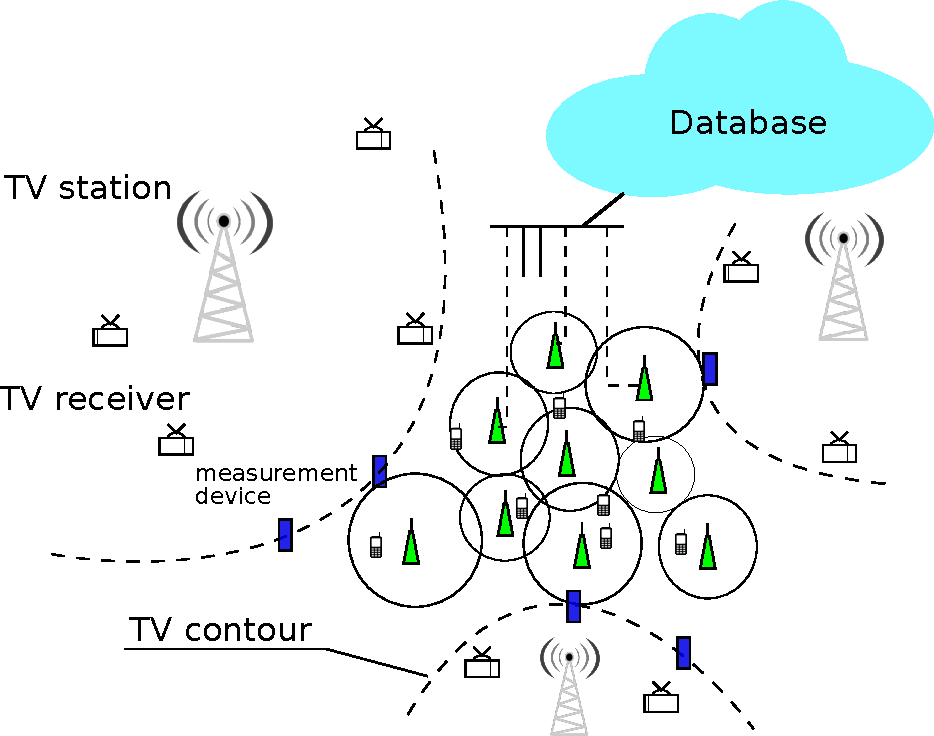
\includegraphics[width=0.9\linewidth]{systemmodel_working.pdf}
  \caption{System model: WBS cells and DTV systems}
\label{sysmodel}
\end{figure}

\subsection{SINR on terminals}
WBSs are interested in payload data communication with their associated terminals. 
As to performance metric for the \gls{QoS} provisioning, we choose the signal to noise and interference ratio (\gls{SINR}) on the terminals.
SINR is the ratio between the received power of signal of interest and the summed interference experienced by the terminal. 
We only focus on the down-link SINR, as the interference caused by uplink communication is neglectable.

Given a WBS $i$, another WBS which works on the same channel is denoted as $\bar{i}$.
As to a certain terminal $m$ associated to WBS $i$, the path losses between $m$ and the serving WBS $i$ and interfering WBS $\bar{i}$ are denoted as $h_{im}$ and $h_{\bar{i}m}$ respectively.
The path loss is dependent on the distance between the corresponding equipments, e.g. $h_{im}=K \cdot d_{im}^{-\alpha}$, where $\alpha$ is the path loss exponent, $d_{im}$ is the distance between $i$ and $m$, $K$ is a constant which models the reference loss over a single unit of distance.  
$N_0$ denotes the thermal noise power.
Shadowing without fading is considered in our model.
The sum of all disturbing radio frequency effects (including interference) on terminal $m$ (we assume the working channel is $c$) is as following,
\begin{equation}
\label{interference}
\begin{aligned}
f_m^c=\sum_{\bar{i}} (P_{\bar{i}}^c \cdot h_{\bar{i}j} \cdot z_{\bar{i}m}) +  N_0
\end{aligned}
\end{equation}
where $P_{\bar{i}}^c$ denotes the transmit power of interfering WBS $\bar{i}$, $z_{\bar{i}m}$ models the zero-mean log-normally distributed shadow fading between $\bar{i}$ and $m$, and the standard deviation is $\sigma_{\text{SH}}$.
%Note that $z$ is dependent on the individual transmitter/receiver pair, but we omit the subscripts for simplicity. 
Then we get the \gls{SINR} on end terminal $m$,
\begin{equation}
\label{SINR}
\begin{aligned}
\gamma_{m} = \frac{P_{i}^c \cdot h_{im}\cdot z_{\bar{i}m}} {f_m^c}
\end{aligned}
\end{equation}



\subsection{Problem Statement}
Our goal is to design distributed solution for WBSs to choose channel and transmission power, so as to improve the SINR on their end terminals.
Each WBS's utility is a function of certain form of the SINR on all its end terminals, \ie the utility can be the average SINR at all its terminals.
When adopting a function of SINR on all terminals as utility, as the terminals are mobile, and they are influenced by many factors, \ie the type of service provided to the terminals, the utility may diverge from the real performance of the terminals.
%Thus, due to the mobility of terminals, it is non realistic to adopt a function of SINR on all terminals.
On the other hand, it is not appropriate to choose one~\cite{spectrum_sharing_tvspace_2012} or more fixed terminals, and use their SINRs to represent the SINR for all the other terminals in that cell, because their location could diverge greatly with the locations of the other terminals.
As a result, we propose a metric \textit{QuasiSINR} to represent WBS's performance, which is independent on the actual locations terminals.

%We are interested in improving the SINR on the terminals of each cell by rendering WBSes to decide their channel and transmission power.
%The distribution of mobile terminals is varying and influenced by many factors, \ie the type of services provided to the terminals, the type of area and mobility of terminals.
%Thus when WBS decides its transmission parameter, it has to evaluate the SINR of all terminals.
%Furthermore, taking into consideration of terminals' SINR makes it very difficult to formulate WBS's preference on resources, \ie channel, power.
%Thus, we propose a simplified metric \textit{quasiSINR} for each WBS, which is independent on any terminals, and is able to  reflects the SINR on a circle around the WBS in a conservative manner.
%QuasiSINR can be easily adjusted by changing the radius of the circle so that the the circle goes through the majority of the terminal users.


\subsubsection*{QuasiSINR of WBS}

QuasiSINR is an indication of SINR that a WBS can provide to its terminals.
Given an auxiliary circle centering at WBS, quasiSINR of a WBS is the ratio between the weakest signal of interest and the summation of the strongest interference caused on the circle.
Figure~\ref{quasiSINRfigure} illustrates how is quasiSINR calculated.
%
The discussed WBS is denoted as $i$, and the rest WBSs are denoted as $j$, $j'$ and $j''$ respectively.
We assume all the WBSs work on the channel $k$, this co-channel interference is caused on each WBS.
An auxiliary dashed circle centering at WBS $i$ is shown, whose radius is $\delta$. 


\begin{figure}[h!]
  \centering
  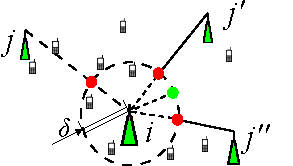
\includegraphics[width=0.6\linewidth]{quasiSINR2.pdf}
  \caption{QuasiSINR is the ratio between the power of signal of interest on the green point with the co-channel interferences on the red points}
\label{quasiSINRfigure}
\end{figure}


The power of the signal of interest on auxiliary circle is,
\begin{equation}
\label{quasiSINR_1}
\begin{aligned}
\tilde{P_i} = P_i\cdot h\cdot z = P_i^c\cdot \delta^{-\alpha}\cdot z
\end{aligned}
\end{equation}	
where $h$ and $z$ are the attenuation and fading from $i$ to any point on the auxiliary circle.
In Figure~\ref{quasiSINRfigure}, $\tilde{P_i}$ is the power of the signal of interest received on the green dot 

The interference on auxiliary circle from co-channel WBS $j$ is,
\begin{equation}
\label{quasiSINR_inf}
\begin{aligned}
\tilde{f_{ji}} = P_j^k\cdot h'\cdot z' = P_j^k\cdot (d_{ji}-\delta)^{-\alpha}\cdot z'
\end{aligned}
\end{equation}
where $h'$ and $z'$ are the attenuation and fading from $j$ to the nearest point on the auxiliary circle.
In Figure~\ref{quasiSINRfigure}, $\tilde{f_{ji}}$ equals to received interfering power from WBS $j$ on the red dot, which is the crossing of the connecting line between WBS $i$ and $j$ and the auxiliary circle.
The sum of interference on the intersections of auxiliary circle and connecting lines is, 
\begin{equation}
\label{quasiSINR_infs}
\begin{aligned}
\tilde{f_{i}} = \sum_{j\in\mathcal{N}, c(j)=k} \tilde{f_{ji}}
\end{aligned}
\end{equation}	
In the following chapter, $\tilde{P}$ and $\tilde{f}$ represent the received power of interest and the strongest interference on the auxiliary circle.
The quasiSINR of WBS $i$ is, 
\begin{equation}
\label{quasiSINR}
\begin{aligned}
 \tilde{\gamma_{i}} & = \frac{\tilde{P_i}^k}{\tilde{f_i}^k + N_0} \\
&=\frac{P_{i}^k \cdot h \cdot z} {\sum_{\tiny\substack{j\neq i, j\in \mathcal{N}\\c(j)=c(i)}} (P_j^k \cdot h' \cdot z') + N_0}\\
&= \frac{P_{i}^k \cdot \delta^{-\alpha}\cdot z} {\sum_{j\neq i, j\in \mathcal{N}} (P_j^k \cdot (d_{ji}-\delta)^{-\alpha} \cdot z') + N_0}
\end{aligned}
\end{equation}

%and we can see QuasiSINR is the ratio between the weakest signal of interest and the summation of the strongest interference.
We can adjust the radius of the auxiliary circle $\delta$ to let WBS foster better service to the terminals in certain area.
For instance, to take care of the SINR on the border area of the cell, the radius $\delta$ can be set as the distance between WBS $i$ and the furthest associated terminal.
When the terminals are close to the WBS, $\delta$ can be set smaller to better fit to the terminals' distribution.
%but it can also be set by operator according to the base station's situation, such as the distribution of end terminals, and the geography of the coverage of the base station. 
%For this terminal furthest away, we now construct a worst-case SINR which factors in all interference from neighboring secondary cells as if they were closest to the considered terminal. Hence, QuasiSINR is the ratio between the weakest signal of interest and the summation of the biggest (possible) interference from other co-channel WBSs. 


%According to this construction, the weakest strength of the signal of interest is $P_i^c\cdot h_{iQ}\cdot z_{iQ} = P_i^c\cdot \delta^{-\alpha}\cdot z_{iQ}$ while the biggest possible interfering power from co-channel WBS $j$ is $P_j^c\cdot h_{jQ}\cdot z_{jQ} = P_j^c\cdot (d_{ji}-\delta)^{-\alpha}\cdot z_{jQ}$. We denote in this context by $Q$ the virtual worst-case terminal.
%%given at a position $Q$ (virtual measurement point) which is $\delta$ distance units away from the serving WBS, and $d_{ij}-e$ distance units away from any WBS $j$ \textit{at the same time}. The received power from WBS $i$ at this virtual measurement point is $P_i\cdot h_{iQ}\cdot z = P_i\cdot e^{-\alpha}\cdot z$, while the received interference power at $Q$ from any co-channel WBS $j$ is $P_j\cdot h_{jQ}\cdot z = P_j\cdot (d_{ji}-e)^{-\alpha}\cdot z$. 
%Hence, as we form the SINR such a virtual 'worst-case' terminal, the co-channel interference impact is overestimated as the total received interference power is given by the sum $\sum_{\forall j}P_j^c\cdot h_{jQ}\cdot z_{jQ}$ where index $j$ spans all co-channel WBSs with $i$. Formally, the QuasiSINR of WBS $i$ is given by:


%any change of the transmit powers of co-channel interference source (i.e. other WBS working on channel $k$) will have always fixed impact to the quasiSINR of the WBS concerned, 
Because of the auxiliary circle, the interaction between co-channel WBSs are independent on the individual end terminals. 
With quasiSINR, the channel and power allocation problem exclude the terminals and simplify the problem. 
%QuasiSINR will be validated in Section \ref{simulation}. 

%Notice regrading the QuasiSINR, that any modification of the transmit powers of co-channel interference source (i.e. other WBS working on channel $c$) will have always the same scaled impact. I.e. we have symmetry among the co-channel interferes regarding their impact on the QuasiSINR. This is the main reason for introducing the QuasiSINR.\todo{?}



\subsubsection*{Calculation Instead of Measurement}
According to our system model, every WBS is able to access the central database which stores all WBSs' geolocations \ie working channel, transmission power, the characteristics of radio frequency environment such as parameters of attenuation and shadowing.
To obtain quasiSINR, we don't need to measure the signal strength, but only need to calculate them based on Formula~\ref{quasiSINR} using propagation model~\cite{Jaentti11} and the information stored in central database.
%Besides, the channel usage of each WBS is also recorded in the data center.
%$h_{ij}$ and $z_{\bar{i}j}$, and also the transmission power of the interfering WBSs. 
%Thus when WBSes work in senseless mode, which can calculate the RSSI from one transmitter to an receiver with proper propagation model (e.g. Formula\ref{interference}\ref{SINR} can be calculated within database) with the geo-location and channel usage information. 
A WBS also knows the interference it causes on the auxiliary circles of other co-channel WBSs via accessing the database.



\subsubsection*{Optimization}
Our goal can be illustrated in the form of an optimization problem.
To ensure fairness, instead of maximizing the sum of quasiSINR of all WBSs, we minimize the sum of inverted quasiSINR. 
	\begin{equation}
\label{problem}
			\begin{aligned}
			& {\text{Minimize}}
			& & \sum_{i\in \mathcal{N}}\frac{1}{\tilde{\gamma_{i}}} \\
			& \text{subject to}
			& & \sum_{k=1}^{|\mathcal{C}|}x_{ik}=1 \\
			& & & P_{min}^c \leq P^c \leq P_{max}^c
			\end{aligned}
		\end{equation}
%XXX Please formalize the constraints, do not simply write 'one node, one channel'\todo{i'll do it!}
%where $\tilde{\gamma_{i}}$ is the QuasiSINR as defined in Equation~\ref{quasiSINR} XXX Always when you reference to a section, a figure, an equation or a table, mention the corresponding word in front of the reference - otherwise the reader does not know, should he reference to a section, an equation etc. - here I put in an 'Equation' for you but check this for the rest of the paper XXX. 
For a WBS, each channel in $\mathcal{C}$ receives different levels of interference from other WBSs working on it.
In order to provide better service to its end users, WBS is liable to choose either the channel permitting higher transmission power or the channel which experiences less interference, or the channel compromising the two factors according to Formula \ref{SINR}.
 Achieving optimal white spectrum allocation in a distributed style is the goal of this work, furthermore, this distributed solution should converge fast and lead to an efficient and stable solution.


%When we look at the power and channel allocation problem in the scope of IEEE 802.22 network, as the restriction on interference generated by the secondary users need considering, the problem illustrates differently.
\section{Related Work}
\label{relatedWork}
%xxxxxxxxxxxxxxx
%%'tvws_paper_networking2015' needs reading.
%Scheduling Variable Rate Links via a Spectrum
%Server, centralized Spectrum Server that
%coordinates the transmissions of a group of links sharing a
%common spectrum.xxxxxx

~\cite{maximum_power_TVWS_dyspan_2011} presents a method to derive location-specific maximum permitted emission levels for white space devices.


After each update, WBS needs to access the data base to retrieve the current channel usage, then they can calculate xxx.

Firstly we introduce the solutions proposed on the utilization of TV white space, which includes regulations, proposed standards and recent research advances.
Secondly we introduce the power and channel allocation schemes proposed for cognitive radio network, and explain the reasons why they are not suitable to solve our problem.
%Thirdly, we introduce other channel allocation schemes, as our solution employs a channel allocation scheme in one procedure.

\subsection{Utilization of TV white space}
In accordance with the regulations of FCC, some prototype applications are proposed in both cellular network~\cite{tvwhite_lte2011, multicell_geo_dyspan11} and WiFi-like network~\cite{whitefi09}.
The secondary users access the centralized data base to get to know which channels can be used, 

Standardization activities are in progress on TVWS utilization, including IEEE 802.22~\cite{802.22} for Wireless Regional Area Networks (\gls{WRAN}), IEEE 802.11af~\cite{802.11af} for WLAN, IEEE 802.15.4m~\cite{802.15.4m} for 802.15.4 wireless networks in TVWS and 802.19.1~\cite{802.19} for coexistence methods among local and Metropolitan Area Networks (\gls{MAN}).

%\cite{HoangPowerChannel2010} proposes a distributed solution for power control and channel assignment in both down-link and up-link communication in a WRAN, but the investigated secondary network is composed with only one base station and multiple terminals.

%% related work!!!
Scientific research on utilization of TVWS goes on in parallel with the regulatory agencies.
Feng et al. ~\cite{hybridPricing_tvspace_2014} investigate the business model of TV spectrum utilization in database involved network structure, emphasis on the price policy of the channels approved by FCC.
Spectrum sharing in TVWS is formulated as a series of optimization problems. 
The guarantee that TV receivers should not be affected by the aggregate interferences form TVBDs is one constraint.
The objective can be maximizing TVBD's downlink transmission power~\cite{multipleIntf_pimrc11}, uplink transmission power~\cite{uplink_power_tvws13}, or best geographic distribution of TVBDs~\cite{withinTVcoverage_PIMRC13}.
\cite{game_CA_association_ICDCS12,SA_CA_TVWS_2012crowncom, 802.22co-existence09, 802.22game_08globecom,self-coexistenceWRAN2010infocom} emphasise on interference mitigation among TVBDs via spectrum allocation.
Vehicular networks operating with TVWS assisted by TV database and cooperative sensing is discussed in~\cite{tvws_vtc13}.
Work~\cite{increaseTVWS12} steps further from the database paradigm and makes efforts to utilize the \textit{grey space}, where TVDB is allowed to operate even within the TV service area.



\subsection{Resource Allocation in CRN}

The proposed solutions can be divided into two categories, centralized and distributed, which will be introduced sequentially.

To implement centralized solutions, optimization problems are often formulated.
In \cite{downlink-centralized-08-TWC}, the objective is to increase the number of supported terminals whose SINRs are above a threshold, and the constrains are to refrain the interference at the primary users within a certain margin.
\cite{joint_power_channel_linkpair_08ICT} minimizes the transmission power and meanwhile makes sure the SINR of terminal is above a threshold, but this work fails to consider the protection of primary users.
A heuristic algorithm is proposed in \cite{centralized_80222_sharing_ifip2011}, which considers the channel availability and transmission demand of each WBS.
%Spectrum allocation is solved after being formulated into a colouring problem.
The aforementioned two schemes don't consider varying the transmission power.
% xxxx important paper
%A centralized scheme is proposed in \cite{nashbargaining_2012jsac} for joint channel and power allocation among end terminals in OFDM cognitive radio network. 

As to decentralized schemes, in order to avoid or to alleviate co-channel interference between cells, and to allow arbitrary number of cells to work in IEEE 802.22 network, \cite{Inter-Network_Spectrum_Sharing_80222_08} proposes distributed inter-network spectrum sharing scheme, where contention decisions are made in a distributed way and the winner cells can use the shared channels.
This work doesn't consider the role of transmission power in the co-channel interference.
%
An distributed power allocation (single channel) scheme based on learning for secondary networks is given in \cite{aggregatedInf_Galindo_crowncom09}, where penalty function involving the interference threshold on primary systems is used.

\cite{HoangPowerChannel2010} discusses power control and channel assignment in both down-link and up-link communication in cellular network. 
Although the solution is distributed, primary users are required to cooperate with secondary base station in a learning process to decide the transmission power, in addition, there is only one secondary base station considered whereas we need to cope with the multiple cells in our problem.
%
Joint channel-power selection for multiple transmission links (pairs) is investigated in \cite{wuinfocom09}. 
The authors decompose the Lagrangian dual of the problem, then propose a distributed scheme based on the dual parameters. 
The scheme converges into pure Nash equilibrium, but in order to facilitate this scheme, monitors are required to watch interference from secondary users, moreover, monitors have to be equipped computational ability and interact with secondary users in the whole process of convergence.
%
A distributed joint power and channel allocation is proposed in~\cite{pimrc_2012}, each base station chooses optimal power level and channel to optimize its utility, which results in induced received interference and caused interference on primary users. 
The execution of this scheme is formulated into an exact potential game. 
For each base station, after several rounds of best responses in terms of channel and power level, Nash equilibrium is achieved.
There are some flaws hindering the application of this scheme.
Firstly, the paper doesn't provide means for base stations to obtain the needed information which is needed to calculate the utility function.
Secondly, it is not clear how to calculate the punishment in the utility function, which indicates whether and how much the interference threshold on primary users is violated.
Thirdly, the convergence speed of the scheme is not given, in fact, as the problem is formulated into a potential game, converge speed or the number of updates before convergence is a theoretic problem which is still unsolved.
Last but not least, as the utility function and the potential in the game are designed as the sum of received and introduced interference, the desired signal power and the punishment, the minimization of this \textit{sum} does indicate meaningful  performance metrics, \ie SINR on terminals, or the total transmission power consumption.
In~\cite{spectrum_sharing_tvspace_2012}, Chen et al. investigate the channel allocation problem in the scenario of TV white space.
The channel allocation problem is formulated into a potential game, individual WBS's utility is to maximize the capacity of one single static terminal.

Potential game is also adopted in work~\cite{tvws_paper_networking2015} to design algorithms, which mitigates the adjacent interference.




\cite{powerChannelAllocation_2015_shapley} adopts cooperation game to research the coexistence of femtocells.
Each femtocell negotiates with neighbouring fremcells, and they form temporary coalition, but the goal of this solution is to allocate resource block in terms of time and transmission power.

%
Distributed algorithm based on Learning is proposed in \cite{cogCE_huang} for LTE to allocate the the resource block in down link, which leads to correlated equilibrium, but slow converge hinters its application.
%
\cite{joint_power_channel_linkpair_08ICT} proposes both centralized and decentralized solutions.
Two distributed schemes are proposed, joint channel and power allocation is formulated into a weighted potential game, as an alternative workaround, the problem is solved in two sequential phases.






\section{Problem Decomposition and Corresponding Related Works}
In the related works, the protection on primary users is taken care during the process where channel and power selection are conducted, but according to the current regulations and standards, there exists no communication means between the secondary users and the primary users.
Besides, assuming such communication media is available, the communication overhead between primary users and second users is considerable.
We decide the maximal transmission power for each WBS on each channel before dealing with channel and power allocation, and this work is conducted at the centralized database.
As the database has global info of the network, it guarantees the primary users are not interfered when all the WBSs work on the same channel.
By decompose the problem into two subproblems, the protection on the primary users from harmful interferences is excluded out of the latter consideration on channel and power allocation.


%We propose a distributed workaround for the join power channel allocation problem, so that 
In summery, we solve the channel and power allocation in downlink communication in IEEE 802.22 network by solving three sequential sub problems:
\begin{itemize}
\item  Firstly, given a set of secondary WBSs and their geo-locations, the maximum permitted transmit power on each channel for each WBS is determined, so that the interference margin can not be exceeded no matter how do WBSs utilize the spectrum and power resources. 
In other words, the dynamics in the secondary network is transparent to the primary system. 
\item Secondly, once the maximal transmit power is determined, each WBS chooses its operating channel, this subproblem is a channel allocation problem with different transmission power. 
\item Thirdly, transmission power is adjusted on the channel which is decided in the previous step.
\end{itemize}
The first subproblem is a centralized approach, the following two problems are solved with distributed schemes.
In the following, we introduce the related works with the corresponding sub problems.

%We discuss the detailed problems in the following two subsections in combination with related work in the respective area.
%XXX Di, how can it be possible that we set the maximum transmit power and let the secondaries choose their operating channel afterwards? Isn't this related to each other ? XXX  
%XXX Answer: I decide the maximal transmission power in a very conservation way: let all of the WBSs work on the same channel and decide the max power. This need strong argument XXX

%In this paper we contribute by addressing this problem from two complementary directions. On the one hand, we study a convex formulation for setting the maximum transmit power at a set of secondary users given different interference margins for primary users. This scheme assumes a central controller to be in place which has geo-information and sufficiently detailed radio maps to characterize the path loss. We show that this convex formulation provides superior performance compared to linear problem formulations proposed in related work. Furthermore, we address the problem of assigning channels to WBS. Here, apart from the resulting cell performance, we also consider convergence of the assignment scheme as well as power consumption as important metrics. We propose a distributed scheme which interacts with a data base to get to know the channel choices of neighboring base stations, the interference relationships as predicted by radio maps as well as the maximal transmit powers. Formulated into a congestion game, the proposed schemes converges fast and provides superior performance in terms of cell performance and power consumption. 



\subsection{Maximal transmission power planning}
\label{MPowerPlanning}
%Secondary network should not interfere TV receivers, thus regulation on transmission power is necessary.
%\cite{Chen_PowerControl,SenhuaHuang10,Zhu09} propose schemes for secondary users to decide the transmission power with sensing technology, one prime consideration of schemes is obviating interfering incumbent primary users. A distributed scheme to adjust power based on learning is proposed in \cite{aggregatedInf_Galindo_crowncom09} for each WBS, where a penalty function involving the interference threshold is used. This scheme needs many steps to converge, and there is no interference margin for network dynamics.
%Solving the joint problem of power and channel allocation in a distributed manner is challenging.
 
 
To protect the TV contours from harmful interference, the aggregate interference caused by WBSs at the contours of TV receivers should be within interference margin~\cite{multipleIntf_pimrc11}.
The sufficient condition in the context of TV white space is formulated into a centralized linear programming program (\gls{LP}).
Adopting centralized scheme is due to the special network structure according to IEEE 802.22 standard. 
The standard requires a centralized database to store the available channels for each secondary base station, thus centralized scheme can be conducted there after trivial modification.
The objective function is to maximize the summation of all secondary base stations' transmission power, and the constraints are formed to satisfy the sufficient condition for every interference measuring device for the TV receivers. %, However, this approach doesn't take the channel assignment problem into account.
%XXX This discussion of the related work is a bit confusing. The problem is that it is no clear per discussed paper what the shortcoming of the approach is. I.e. you describe the approaches but you do not help the reader why this approach is not contributing to the goal defined in the first sentence. Try to reformulate this section more precisely expressing what is the problem with the corresponding approach XXX.



\subsection{Channel allocation with fixed transmission power level}
\label{CA}
After knowing the maximum transmission power on each channel, WBSs need to decide which channel to use so as to mitigate interference among WBSs and provide the best SINR for their end users. 
Here we assume WBSs' transmission power is the maximum permitted and fixed.

This problem lies in the category of \textit{channel assignment problem}, which has been well investigated in many scenarios.
Channel assignment problem tries to mitigate co-channel interference among users, which can be converted into colouring problem thus is NP hard~\cite{Hyacinth}. 
Authors of~\cite{Ko_DistributedCA} propose heuristic algorithms utilizing best response to improve its welfare, but the transmission power is assumed identical and path loss is deemed as symmetric, which renders this method problematic for our problem where transmission is non-identical and the path loss is asymmetric.
\cite{CApotentialLearning_05dyspan} formulates channel assignment problem in ad-hoc cognitive radio network into potential game which leads to pure NE, a learning scheme achieving slightly better performance is provided for comparison, but they assume the transmission power is identical and there is no noise in the secondary network, and the proposed random access mechanism demands a huge amount of information to be exchanged, which is a burden for network in ad-hoc structure.
\cite{CA_Felegyhazi_07infocom, Wu_GOP_CA_08infocom} investigate the channel allocation problem under game framework in same collision domain, the authors propose algorithms to converge to pure Nash equilibrium (NE) and strongly dominate strategy equilibrium respectively. 
%\cite{whitefi} discusses channel assignment in the domain of white space, while, it deals with the temporal and spatial existence of spectrum availability where AP and clients choose the same chunk of channels based on spectrum capacity, and leave the interaction among APs unconsidered.
As to our knowledge, there is no work dealing with channel allocation with such asymmetric interactions. 
%XXX So here we have the same problem as above: Only for the first two papers you say explicitly what problems come up with them - for the rest you simply mention them and their approach. Here we really need a much more clearer formulation of the shortcomings - why are they failing to be a solution to our problem ? Furthermore, there seem to be quite a lot of work in game theory and power control in secondary networks - how do they relate to our work? XXX


XXXXXXXXXXXXXXXXXXXXXXXXXXXXXXX

%Channel allocation facilitates CRN to improve throughput~\cite{channelAllocation_throughput_12wcnc}, or cooperatively relay~\cite{channelAllocation_relay_2010ICASSP} and so on.
%This thesis emphasises on co-channel interference mitigation with distributed channel allocation. 

Mitigating co-channel interference via channel allocation has been attracting plenty of research efforts in the past decade, from multiple channel mesh network~\cite{Hyacinth}, Ad hoc network~\cite{Ko_DistributedCA} up to cognitive radio network~\cite{SA_CA_TVWS_2012crowncom,qlearning_huang}. 
Channel allocation problem is converted into colouring problem thus is NP hard~\cite{Hyacinth}, thus centralized optimization fails to produce.
Authors of~\cite{Ko_DistributedCA} propose heuristic algorithms utilizing best response based on the welfare on itself to assign channels among users.
Simulated annealing is applied to mitigate co-channel interferences in~\cite{SA_CA_TVWS_2012crowncom}.
For the same purpose, no-regret learning~\cite{qlearning_huang, hart00correlatedeq} is exploit to optimize the choice on channel.
All the available channel allocation schemes are designed under the same assumption, that the transmission power levels are identical, and the attenuation between any pair is reciprocal.
\subsection{Power allocation}
\label{PA}
Working with the maximal permitted transmission power may not be the optimal in terms of power consumption and the SINR on terminals.
Thus distributed power adjustment is conducted.

We name the our solution of channel and power allocation as \gls{DiCAPS} (Distributed Channel Allocation and Power Selection), and call the solution to a sub-problem of it, \ie channel allocation, as \gls{WhiteCat} (White space Channel allocation).

%In this work we concern the best possible quality-of-service provisioning by allocating channels on which fixed transmission power is used.
%In this paper we try to improve the SINR on secondary end terminals through WBSs' power-channel strategy. To facilitate analysis and proposition of solution, we propose a metric \textit{QuasiSINR} for each secondary base station to represent the SINR of the terminals in the coverage of that base station.


%\todo{todo:}
%\begin{itemize}
%\item what is the reason to design a distributed scheme for this problem.
%\begin{itemize}
%\item complexity (to w)
%\item overhead
%\item WBSs belong to different commercial organization (we actually propose a spectrum sharing paradigm)
%\end{itemize}
%
%\item argument 1: why is the utility used in the algorithm, in other words, what is the reason to chose it and what is the relation between it and the SINR on end users.
%
%\end{itemize}




\section{The Maximum Permitted Transmission Power}
\label{powermap}
The WBSs work in underlay manner with primary TV stations, the aggregate generated interference on each channel should not excess the threshold of the interference measuring devices.
We adopt the interference model and the optimization methodology from the work of \cite{multipleIntf_pimrc11} to plan the maximum transmission power on each channel for WBSs.
%XXX Why is exactly this approach adopted ?XXX.
%\todo{describe\\ the\\ interference\\ model\\ of [14]} 
Having a global view of the propagation parameters, geolocations of WBSs and interference threshold at interference measuring devices, linear programming is implied in the database to calculate the maximum permitted power.

For WBS $i\in \mathcal{N}$, the maximum transmission power allowed on channel $c$ is denoted as $P_i^c$. 
As to each channel $c\in \mathcal{C}$, the generated interference on each interference measuring device should be within a predefined interference margin $I^c_{pt}$.
The interference margin in a slow fading environment is decided according to~\cite{aggregate_interference_shadow_fading_2010}.

Then the maximum permitted transmission power on channel $c$ for each WBS can be obtained by solving the following optimization problem,
	\begin{equation}
\label{lp}
		\begin{aligned}
		& {\text{Maximize}}
		& & \sum_{i\in \mathcal{N}} P^c_i \\
		& \text{subject to}
		& & \sum_{i\in \mathcal{N}} (P^c_i \cdot h_{i,pt}\cdot z) < I^c_{pt},\\
		& & & P_{min}^c \leq P_i^c \leq P_{max}^c		
		\end{aligned}
	\end{equation}
	
%	XXX I am wondering here: You already define the solution in this section rather than defining the problem as indicated in the section title - why do we need to introduce here the solution ?XXX

$P_{min}^c$ is the prudent transmission power by FCC, we set is as 4 W. 
$P_{max}^c$ is the maximum transmission power.
$z$ is shadow fading as introduced in \ref{SINR}.
Here we only consider the interference caused by WBSs, and omit the interferences from end terminals. 
Since WBSs' transmission power is higher and their altitude is higher\cite{multipleIntf_pimrc11}, thus the downlink transmission contributes the major part of interference\cite{infmitigate07mobicom}.
%, in contrary the interference caused by end terminals is trivial and omitted. 
The first constraint indicates that the interference margin will not be exceeded even when all the WBSs work on the same channel.


Formula~\ref{lp} will be solved for each channel $c\in \mathcal{C}$.
%There will be multiple constraints for \ref{cvx} if there are multiple DTV contours working on channel $c$. 
After solving the $|\mathcal{C}|$ problems, the maximum permitted transmission power vector $\bm{P^c} =\{P_1,\cdots,P_{|\mathcal{N}|}\}, \forall c\in \mathcal{C}$ is obtained.
%We solve this convex optimization problem with \cite{cvx} in the centralized base station.

If implying linear programming to decide the maximal transmission power, the WBSs locating far from TV coverage cell border
contribute more to the aggregate of power with the biggest permitted power, as a result the maximal transmission power on each channel obtained with LP is seriously unbalanced.
To address this fairness issue, we maximize the summation of the logarithmic value of every WBS's value, then for each channel $c\in \mathcal{C}$, we formulate the problem into a convex optimization problem.

	\begin{equation}
		\label{cvx}
		\begin{aligned}
		& {\text{Maximize}}
		& & \sum_{i\in \mathcal{N}} \log P^c_i \\
		& \text{subject to}
		& & \sum_{i\in \mathcal{N}} (P^c_i \cdot h_{i,pt}\cdot z) < I^c_{pt}, 
		\end{aligned}
	\end{equation}


Figure \ref{lpcvx} depicts the distribution of maximal transmission power levels obtained in 100 simulations. In each simulation the locations of TV contours are randomly decided around the WBSs. It can be seen that around half of WBSs' transmission power planed with LP is restricted to be the minimum transmission power, and the other half of WBSs' transmission power is the maximum permitted power. By applying convex programming, the planed maximal transmission power levels are distributed evenly in between the minimum and maximum permitted power. The gain of SINR on end terminals by applying convex optimization to decide the maximal transmission power is illustrated in the simulation section.

\begin{figure}[h!]
  \centering
  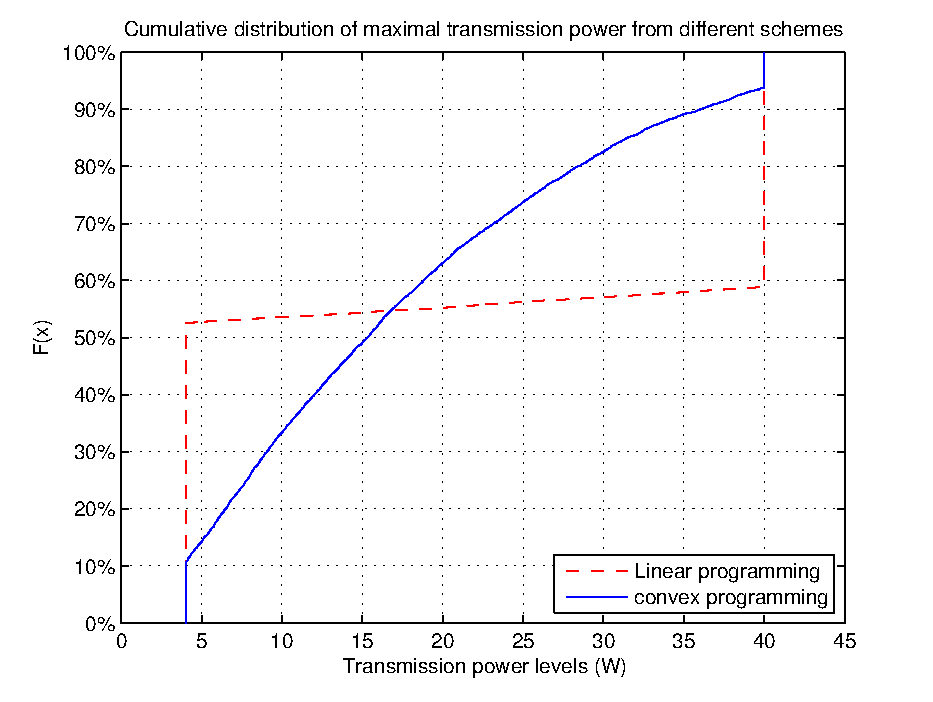
\includegraphics[width=0.89\linewidth]{lpcvxcdf100runs.pdf}
  \caption{Distribution of maximal transmission power levels obtained from convex and linear programming respectively}
\label{lpcvx}
\end{figure}


Optimization problem \ref{cvx} provides the maximal transmission power without violating the TV contour, as there are multiple channels available in the network, as long as there are WBSs which work on a different channel from others, there will be a new interference margin for TV contour, which provides tolerance space for network dynamics such as new WBS starting to work or increased interference on TV contour because of variance of broadcast path condition. 
%XXX As mentioned above, it is not clear which impact the relationship between maximum transmit power planning and channel selection has XXX.


\section{Channel Allocation with Fixed Transmission Power}
\label{CA_fixedPower_2subproblem}
%As discussed in~\ref{CA}, there is 
First, we give the centralized solution, then the decentralized scheme is introduced.
\subsection{Centralized optimization programming}
In the very beginning, we formulate the channel allocation problem into a binary quadratic programming problem which can be solved in a centralized way.  For two nodes $i$ and $j$, there is,
\begin{equation}
\begin{split}
X_i^TX_j = \sum\limits_{k=1}^{|\mathcal{C}|}x_{ik}\cdot x_{jk} = 
\left\{ \begin{array}{ll}
1 & \mbox{if $c_i=c_j$} \\
0 & \mbox{if $c_i\neq c_j$} 
\end{array}
\right.
\end{split}
\end{equation}

The power levels across all channels are denoted by a constant vector $P^{|\mathcal{C}|\times 1}$, which possibly nonidentical to all nodes because of maximal channel planning. The power used by user $i$ is $P_i^TX_i = \sum\limits_{k=1}^{|\mathcal{C}|}P_{i}^k\cdot x_{ik}$.


Problem \ref{problem} can be modeled via general purpose nonlinear optimization:
	\begin{equation}
\label{QLP}
		\begin{aligned}
		& \underset{}{\text{minimize:}}
		& & \sum\limits^{n}_{i=1} \frac{\sum\limits_{j\in\mathcal{N}, j\neq i}P^TX_j(X_j^TX_i)h_{ji}z + N_0}{P^TX_i}\\
		& \text{subject to}
		& & \sum\limits_{k=1}^{|\mathcal{C}|}x_{ik}=1, x_{ik}\in X_i\in \{0,1\}^{|\mathcal{C}|}\\
		\end{aligned}
	\end{equation}
$x_{ik}$ with $i\in \mathcal{N}, k=1,2\cdots$ is binary variable. Problem \ref{QLP} is a non-linear problem with binary variables, but it can be reformulated in to a quadratic programming problem as,
	\begin{equation}
\label{QLP_2}
			\begin{aligned}
			& \underset{}{\text{minimize}}\\
			&\sum\limits^{n}_{i=1}(\sum\limits_{j\in\mathcal{N}, j\neq i}\sum\limits_k \frac{P_{j}^k}{P_{i}^k}\cdot h_{ji}\cdot z\cdot x_{jk}\cdot x_{ik} + \sum\limits_k \frac{N_0}{P_{ik}}\cdot x_{ik})\\
			& \text{subject to:} 
			\sum\limits_{k=1}^{|\mathcal{C}|}x_{ik}=1, x_{ik}\in X_i\in \{0,1\}^{|\mathcal{C}|}\\
			\end{aligned}
		\end{equation}

The reformulation is available in Appendix \ref{optdeviation}. We use LINDO~\cite{lindo} which is a state of art non-linear problem solver to solve the problem, which employs Branch-And-Reduce method to get the global optimal for the problem. % We use the results obtained by solving this QLP problem as one reference in the coming section. 
The result will be used as a reference in the simulation section with other schemes. 



\subsection{Distributed White Space Channel Allocation (WitheCat): Algorithm and Protocol}
\label{whitecat}
In this chapter a distributed scheme for WBSs to allocate channels is proposed,  which is named as \underline{white} space \underline{c}hannel \underline{a}llocation \underline{t}echnology (WitheCat). WitheCat is depicted by algorithm \ref{whitecatalgo} which is a best response process, where each WBS (referred as $i$) greedily searches for a preferred channel based on utility function $u_i$, and the sum of all WBSs' utilities is minimized after finite times of updates even the interaction between WBSs are asymmetric. The utility is as follows,

\begin{equation}
\label{utility}
u_i =\dfrac{\sum\limits_{\tiny\substack{j\in \mathcal{N}, j\ne i,\\ c(\sigma_j)=c(\sigma_i)}}\tilde{f_{ji}}}{2\cdot \tilde{P_i}} + \dfrac{1}{2}\sum_{\tiny\substack{j\in \mathcal{N}, j\ne i,\\ c(\sigma_j)=c(\sigma_i)}}\dfrac{\tilde{f_{ij}}}{\tilde{P_j}} + \sum_{\tiny\substack{\mathcal{S}:i,j\in \mathcal{S},\\ c(\sigma_j)=c(\sigma_i)}}\dfrac{N_0}{C\cdot \tilde{P_i}}\\
\end{equation}
where $\tilde{f_{ij}}= P_i\cdot h_{ij}\cdot z$ and $\tilde{f_{ji}}= P_j\cdot h_{ij}\cdot z$.
Overlooking the constant coefficient 2, the first item of $u_i$ is one part of the inversed QuasiSINR of station $i$. To minimize the first item, WBS $i$ needs to choose a channel either permits larger transmission power or experiences less interference, whereas the larger power will increase the second item which is part of inversed QuasiSINR of other co-channel WBSs. Hence, the cost function presents a reasonable comprise between the welfare of one WBS and others. If WBS only emphasizes on its own utility (e.g. the first part of Formula \ref{utility}), the best response process doesn't converge. We have following theorem:
\begin{theorem}
\label{noconvergence}
\emph{With non-identical transmission power, if every WBS updates its channel based on algorithm \ref{whitecatalgo} with utility based on its own interests, the process doesn't always converge.}
\end{theorem}
The proof is in Appendix \ref{proof}.


\begin{algorithm}[!h]
\caption{Spectrum selection by node $i$}          % give the algorithm a caption
\label{whitecatalgo} 
\KwIn{$d_{ij}$: the distance between interfering WBS $i$ to the auxiliary circle of WBS $j$ for $\forall i, j\in \mathcal{N}$; path lose between $i$ and any other WBS $h_{ij}$, $j\in \mathcal{N}, j\neq i$, and the fading $z$ on it; noise $N_0$; total number of secondary base stations $N$; maximal transmission power $P_j^c, j\in \mathcal{N}, c\in \mathcal{C}$;
$c(j)$, current channel used by $j\in \mathcal{N}, j\neq i$.
}
%\KwOut{a channel }
\For{$i\in \mathcal{N}$}
{\For{$c\in \mathcal{C}$}
{
 calculate $u_i(c)$ based on Formula \ref{utility}\\
 \eIf{$u_i(c)<u_i(c(i))$}{$c(i)\leftarrow c$}{$c(i)$ unchanged}
}
Notify data base of its channel usage, which notifies the other WBSs
}
\end{algorithm}

$c(i)$ is the current channel used by $i\in \mathcal{N}$. Imitating the player's behavior in the congestion game, each base station tries to find the channel $c\in \mathcal{C}$ that brings the smallest $u_i$ based on the other stations' decisions, every channel update will decrease the summation of utilities in the whole network and finally converges to a pure Nash equilibrium (proof is in section \ref{game}.


Some parameters needed to calculate the utility are identical for all WBSs, such as quasi distance $e$, the total number of WBSs $N$, number of channels $C$, attenuation factor $\alpha$, standard deviation $\sigma_{WBS}$ in flat shadowing and noise $N_0$, albeit the following information is further needed to calculate $u_i$: 
	\begin{itemize} %{labelitemi}{$\bullet$}
	\item $\sum_{\tiny\substack{j\in \mathcal{N}, j\ne i,\\ c(\sigma_j)=c(\sigma_i)}}\tilde{f_{ji}^c}, c\in \mathcal{C}$: the received interference on $i$' virtual measurement point from other WBSs $j$ working on the same channel for $\forall c\in \mathcal{C}$.
	\item $\tilde f_{ij}^c$: the interference caused by $i$ on $j$'s virtual measurement point when $i$ works on channel $\forall c\in \mathcal{C}$.
	\item $P_j^c$: transmission power of $j$ for using $\forall c\in \mathcal{C}$.
	\end{itemize}
Unfortunately, it is difficult to get these interferences of interested measured, for station $i$, it is low efficient to scan all channels and obtain the interferences $f_{ji}$ on virtual measurement point for each channel, furthermore, it is impossible to split the interference $f_{ij}$ from the total interference received on WBS $j$' virtual measurement point. 

Enlightened by the work of \cite{SenseLess2011} which verifies the usage of geolocation information in deciding the available channels, we let every WBS store the location information and maximal power map of all other WBSs, and it retrieves information about channel usage by other WBSs from centralized base station, after executing Algorithm \ref{whitecatalgo}, it reports to centralized base station of its channel update. As the location of WBSs and TV stations and the transmission channel and power of TV stations are usually static (entries of TV station change averagely once in 2 days\cite{SenseLess2011}), except for the channel usage in the network, the change of the other data stored in WBS is infrequent. 


We refer \cite{CApotentialLearning_05dyspan} to decide the sequence for WBSs to update their channel. \cite{CApotentialLearning_05dyspan} proposes a method like random access mechanism of CSMA/DA, where the access for broadcast medium is changed to getting access to the centralized center to retrieve the current channel usage and update its new channel. All WBSs are able to access the database in one round (with random or predetermined sequence). As WBSs are connected with database, the control messages needed to decide the sequence will not become a burden. Update of channels can happen in the boot phase, or when the quality of services (the SINR on its end users) of WBSs falls below a threshold, or a fixed time duration comes to end, or a new WBS joins in the network. 


\subsection{Analysis in game theoretical framework}
\label{game}
We give an elegant proof on WhiteCat's convergence in the framework of congestion game theory. Formulating a spectrum sharing problem into a congestion game and the concept of \textit{virtual resources} are firstly proposed in \cite{allerton08_liu} which 'reversely engineer' the distributed channel allocation schemes proposed in \cite{babadi_08, Ko_DistributedCA}.

%\subsubsection{Congestion Game}
%A congestion game \cite{Rosenthal}\cite{Voecking06congestiongames} can be expressed by a tuple $\lambda=(\mathcal{N},\mathcal{R},(\sum_i)_{i \in \mathcal{N}},(g_r)_{r\in \mathcal{R}})$, where $\mathcal{N}=\left\{1,\ldots,N\right\}$ denotes the set of players (each each is labeled with a unique index number), $\mathcal{R}=\left\{1,\ldots,m\right\}$ the set of resources, $\Sigma_{i\in\mathcal{N}} \subseteq 2^{\mathcal{R}}$ is the strategy space of player $i$. Under strategy profile $\sigma=(\sigma_1,\sigma_2,\cdots \sigma_N)$, player $i$ chooses strategy $\sigma_i\in \Sigma_i$, and the total number of users using resource $r$ is $n_r(\sigma)=|\{i\mid r\in \sigma_i\}|$. The cost $g_r: \mathbb{N}\rightarrow \mathbb{Z}$ is a function of the number of users for resource $r$, $g_r^i=\sum_{r\in \sigma_i} g_r(n_r(\sigma))$. In our paper, $g_r^i$ is referred as \textit{congestion} and is Monotonic.
%
%Rosenthal's potential function $\phi:\sigma_1\times\sigma_2\times\cdots\times\sigma_n\rightarrow Z$ is defined as:
%\begin{equation}
%\label{4}
%\begin{split}
%G(\sigma) 
%& =\sum\limits^{}_{r\in \mathcal{R}} \sum\limits^{n_r(\sigma)}_{i=1} g_r(i)\\
%& =\sum\limits_{i\in \mathcal{N}} \sum\limits^{}_{r\in \sigma_i} g_r(n_r^i(\sigma))\\
%\end{split}
%\end{equation}
%$n_r^i(\sigma)$ means the number of players using resource $r$ and \textit{their indices are smaller than or equal to $i$}. Note that the potential is \textit{not} the sum of congestions experienced by every user. The change of the potential caused by one player's unilateral move from $\sigma$ to $\sigma'$ is equivalent to the change of gain (or loss) of that player.
%\begin{equation}
%\label{5}
%\varDelta G(\sigma_i \rightarrow \sigma_i') = g^i(\sigma_i',\sigma_{-i}) - g^i(\sigma_i,\sigma_{-i})
%\end{equation}
%$\sigma_{-i}$ is the strategy profile for all players except for $i$.
%As every congestion game is a potential game, and the total potential is finite, thus the number of improvements is upper-bounded by $2\cdot\sum\limits^{}_{r\in \mathcal{R}} \sum\limits^{n_r(\sigma)}_{i=1} g_r(i)$ \cite{Voecking06congestiongames}.
%
%
In congestion game, each player acts selfishly and aims at choosing strategy $\sigma_i\in \Sigma_i$ to minimize their individual cost.
The gain (loss) caused by any player's unilateral move is exactly the same as the gain (loss) in the potential, which may be viewed as a global objective function. For problems where the potential of the problem is the same with the summation of the cost of all users, the cost function can be used as a utility function directly. This equivalence doesn't exist in our problem, but by carefully choosing the cost function for players, we can make sure that the change of individuals' cost is in the same direction with that of the global utility.


\subsubsection*{Bridging the game and practical scheme}
\label{gameforproblem}
We utilize the conception of virtual resource which is firstly introduced in \cite{allerton08_liu}. In the following text, we use player and base station interchangeably.

\begin{itemize}
\item Player $i$' strategy space is $\Sigma_i=\{(i,j,c), j\in \mathcal{N}, j\ne i, c(\sigma_j)=c, c=1,2,\cdots,N\}$, and $i$ has $C$ admissible strategies, one strategy related with channel $c\in\mathcal{C}$ is described by the set of virtual resources it uses: $\sigma_i=\{(i,j,c), j\in \mathcal{N}, j\ne i, c(\sigma_j)=c\}$, note that virtual resource $(i,j,c)\neq(j,i,c)$.

\item Under the strategy profile $\sigma=(\sigma_1, \sigma_2, \cdots \sigma_N)$, player $i$ obtains a total cost of 

	\begin{equation}
\label{6}
		\begin{split}
		g^i(\sigma)=
		& \sum\limits^{}_{\tiny\substack{j\in \mathcal{N},j\neq i,\\ c=c(\sigma_i)=c(\sigma_j)}} (g_{(i,j,c)}(n_{(i,j,c)}(\sigma))+g_{(j,i,c)}(n_{(j,i,c)}(\sigma))
		\end{split}
		\end{equation}
\end{itemize}

The transmission power over all channels of player $i$ is $\{p_{i1}, p_{i2},\cdots, p_{i|\mathcal{C}|}\}$ and fixed. Path loss is assumed reciprocal: $h_{ij}=h_{ji}$, but nor is the flat fading $z$. To keep the formula clear in the following part, we denote $\tilde{f_{ij}}= P_i\cdot h_{ij}\cdot z$, $\tilde{f_{ji}}= P_j\cdot h_{ij}\cdot z$, $\tilde{P_i}=h_{iQ}$ for $i\in \mathcal{N}$, where $h_{ji}=h_{ij}=(d_{ji}-e)^{-\alpha}, h_{ii}=h_{jj}=e^{-\alpha}$, $d_{ji}$ is the distance between base station $i$ and $j$, and $\delta$ is the quasi distance introduced in section \ref{SystemModel}. $N_0$ is noise which is identical for any channel and any WBS. We define the cost function for virtual recourses $(i,j,c)$ as follows,
\begin{equation}
\label{costfuc4resrc}
\begin{split}
g_{(i,j,c)}(k) = 
\left\{ \begin{array}{ll}
%\tilde{f_{ji}}/(2\tilde{P_i}) + f_{ij}/(2\tilde{P_j}) + N_0/(C\cdot \tilde{P_i})\\\\
%=\dfrac{P_j\cdot h_{ji}\cdot z/2 + N_0/C}{P_i\cdot h_{iQ}\cdot z} +\dfrac{P_i\cdot h_{ij}\cdot z/2}{P_j\cdot h_{jQ}\cdot z} & \mbox{if $k=2$} \\
\dfrac{\tilde{f_{ji}}}{2\tilde{P_i}} + \dfrac{\tilde{f_{ij}}}{2\tilde{P_j}} + \dfrac{C\cdot N_0}{N\cdot \tilde{P_i}} & \mbox{if $k=2$} \\
%=\dfrac{P_j\cdot h_{ji}\cdot z/2 + N_0/C}{P_i\cdot h_{iQ}\cdot z} +\dfrac{P_i\cdot h_{ij}\cdot z/2}{P_j\cdot h_{jQ}\cdot z} & \mbox{if $k=2$} \\
0 & \mbox{otherwise}
\end{array}
\right.
\end{split}
\end{equation}


As resource $(i,j,c)$ only lies in the strategy space of player $i$ and $j$, and can only be accessed by the two players.
More specifically, according to Formula~\ref{costfuc4resrc}, the cost of resource $(i,j,c)$ is only decided by the number of players using it, which is either 0 or 2.
At the first glance, this is a player specific congestion game, as $g_{i,j,k}$ is decided by the transmission power, inference which are associated with players $i$ and $j$, but not other players.
But the resource ${i,j,k}$ excludes the players except for $i$ and $j$ from using it, and thus the cost happened on this resource is only dependant on how many of players from the set $\{i, j\}$ to use it, thus the cost is a function of the number of players using the resource.

Substitute Formula \ref{costfuc4resrc} to Formula \ref{6}, we get the total cost for user $i$ under strategy profile $\sigma$. 

\begin{equation}
\label{cost1player}
\begin{split}
g^i(\sigma)
%& = \sum_{\tiny\substack{j\in \mathcal{N}, j\ne i,\\ c=c(\sigma_j)=c(\sigma_i)}} g_{(i,j,c)}(2) + \sum_{\tiny\substack{j\in \mathcal{N}, j\ne i,\\ c=c(\sigma_j)=c(\sigma_i)}} g_{(j,i,c)}(2)\\
& = \sum_{\tiny\substack{j\in \mathcal{N}, j\ne i,\\ c=c(\sigma_j)=c(\sigma_i)}} (g_{(i,j,c)}(2) + g_{(j,i,c)}(2))\\
%& = \sum_{\tiny\substack{j\in \mathcal{N}, j\ne i,\\ c(\sigma_j)=c(\sigma_i)}} (\dfrac{\tilde{f_{ji}}/2 + N_0/C}{\tilde{P_i}} + \dfrac{\tilde{f_{ij}}/2}{\tilde{P_j}})\\
& = \sum_{\tiny\substack{j\in \mathcal{N}, j\ne i,\\ c(\sigma_j)=c(\sigma_i)}}(\dfrac{\tilde{f_{ji}}}{\tilde{P_i}} + \dfrac{\tilde{f_{ij}}}{\tilde{P_j}}+ \dfrac{C\cdot N_0}{N}(\dfrac{1}{\tilde P_i}+\dfrac{1}{\tilde P_j})) \\
& = \dfrac{\sum\limits_{\tiny\substack{j\in \mathcal{N}, \\j\ne i,\\ c(\sigma_j)=c(\sigma_i)}}\tilde{f_{ji}}}{ \tilde{P_i}} + \sum_{\tiny\substack{j\in \mathcal{N},\\ j\ne i,\\ c(\sigma_j)=c(\sigma_i)}}\dfrac{\tilde{f_{ij}}}{\tilde{P_j}} + \dfrac{CN_0}{N}\sum_{\tiny\substack{j\in \mathcal{N},\\ j\ne i,\\ c(\sigma_j)=c(\sigma_i)}}(\dfrac{1}{\tilde{P_i}}+\dfrac{1}{\tilde{P_j}})\\
& = \dfrac{\sum\limits_{\tiny\substack{j\in \mathcal{N}, j\ne i,\\ c(\sigma_j)=c(\sigma_i)}}\tilde{f_{ji}}}{ \tilde{P_i}} + \sum_{\tiny\substack{j\in \mathcal{N}, j\ne i,\\ c(\sigma_j)=c(\sigma_i)}}\dfrac{\tilde{f_{ij}}}{\tilde{P_j}} + \dfrac{2CN_0}{N}\sum_{\tiny\substack{i\in\mathcal{S}\subset\mathcal{N},\\\mathcal{S}:\forall i\in \mathcal{S}\\ c(\sigma_i)=c}}\dfrac{1}{\tilde{P_i}}\\
\end{split}
\end{equation}

Let $\mathcal{S}$ denote the set of WBSs which work on the same channel.
Now we try to get the potential over all WBSs, note that the summation of one WBS's congestion is related to its index. For any two WBS $i,j\in \mathcal{S}$ with $i<j$, the potential brought in by $i$ is 0, while, that caused by $j$ is in the form of $g_{(i,j,c)}(2)+g_{(j,i,c)}(2)$. In other words, for each interfering pair of WBSs, only the WBS with bigger index contributes to the potential. The total potential is, 
\begin{equation}
\label{allPotential}
\begin{split}	
G(\sigma) 
& =\sum\limits^{}_{r\in \mathcal{R}} \sum\limits^{n_r(\sigma)}_{i=1} g_r(i)  =\sum\limits_{i\in \mathcal{N}} \sum\limits^{}_{r\in \sigma_i} g_r(n_r^i(\sigma))\\
%& = \sum\limits_{i\in \mathcal{N}}\dfrac{\sum\limits_{\tiny\substack{j\in \mathcal{N}, j\ne i,\\ c(\sigma_j)=c(\sigma_i)}}\tilde{f_{ji}}}{\tilde{P_i}} + \sum\limits_{\tiny\substack{\mathcal{S}\backepsilon i, \mathcal{S}\subset \mathcal{N},\\ \forall j\in \mathcal{S}, j\neq i,\\ c(\sigma_j)=c(\sigma_i)}}  (\dfrac{\mid\mathcal{S}\setminus 1 \mid}{C} \frac{N_0}{\tilde{P_i}})
& = \sum\limits_{i\in \mathcal{N}}\dfrac{\sum\limits_{\tiny\substack{j\in \mathcal{N}, j\ne i,\\ c(\sigma_j)=c(\sigma_i)}}\tilde{f_{ji}}}{\tilde{P_i}} + \dfrac{CN_0}{N}\sum\limits_{\tiny\substack{\mathcal{S}\subset \mathcal{N},\\ \forall i\in \mathcal{S}, c(\sigma_i)=c}} \mid \mathcal{S}\mid   \sum\limits_{\tiny\substack{i\in \mathcal{S}}}\frac{1}{\tilde{P_i}}
\end{split}
\end{equation}



%Question:
%
%When power is variable, is it still a congestion game, or potential game?

When players minimize their utilities (cost or potential) illustrated by Formula \ref{cost1player}, the total congestion in the secondary network given by Formula \ref{allPotential} decreases monotonically before reaching one Nash equilibrium. Players' greedy update in the game to minimize its cost Function\ref{cost1player}, which ceases finally in pure Nash Equilibrium. The strategy and cost function of players in the game is transplanted as Algorithm \ref{whitecatalgo} and utility Function \ref{utility} respectively.

\subsubsection*{Gap between equilibrium and the aimed variable}
Here rises a question, is the final value obtained by Algorithm \ref{whitecatalgo} exactly the same as the expression \ref{allPotential} representing a Nash equilibrium? The answer is that there is very little difference if interference is considered.
Recall the target objective we want to minimize in Problem \ref{problem} is,
\begin{equation}
\label{compare}
\begin{split}	
\sum_{i\in \mathcal{N}}\dfrac{\tilde{f_i}}{\tilde{P_i}}
& = \sum\limits_{i\in \mathcal{N}}\dfrac{\sum_{\tiny\substack{j\in \mathcal{N}, j\ne i,\\ c(\sigma_j)=c(\sigma_i)}}\tilde{f_{ji}}+N_0}{\tilde{P_i}}\\
& = \sum\limits_{i\in \mathcal{N}}\dfrac{\sum_{\tiny\substack{j\in \mathcal{N}, j\ne i,\\ c(\sigma_j)=c(\sigma_i)}}\tilde{f_{ji}}}{\tilde{P_i}} + \sum\limits_{i\in \mathcal{N}}  (\dfrac{N_0}{\tilde{P_i}})\\
\end{split}
\end{equation}
Compare Formula \ref{compare} and \ref{allPotential}, we find that the difference between the objective value and the final value promised by congestion game is the difference between the last items in Formula \ref{compare} and \ref{allPotential}. When channels are evenly distributed, there is $C/N*\mid \mathcal{S}\mid\approx 1$, thus Formula \ref{compare} and \ref{allPotential} are approximately the same, but monotonicity on the decrease of expression \ref{compare} is not perceived whereas convergence to NE is still guaranteed. When $N_0=0$, the potential is exactly the same with the object we want to minimize.

From above analysis, we can see the assumption that each WBS only occupies one channel can be easily removed.
If we regard one WBS as multiple ones which locate at the same place, and each WBS works on one distinct channel, then the proof on convergence of WhiteCat can be applied directly to this case.

Note that the convergence of the game is independent on the the concrete form of the cost function. The reason we use function \ref{cost1player} is the total potential of the game is approximately the same with the total utility of all WBSs in the network, if the the goal of a problem varies and the total utility is different, a distinctive utility for each WBS should be accordingly proposed. Hence, we say that WhiteCat scheme provides a prototype for the problems where the interaction among users are asymmetric: based on a suitable utility involves the welfare of itself and its neighborhood community, the best response approach can converge in a decentralized style.


\subsection{Communication overhead of DiCAPS in the phase of channel allocation}

Channel allocation with different transmission power is NP hard, this is one reason for us to propose distributed algorithm.
DiCAPS is a distributed scheme but certain information of the other WBSs is needed.
The centralized base station is piggybacked to provided the needed information.
As to a WBS, the number of such inquiries is the number of steps before convergence.
The upper bound of total update steps is $2n^2$, thus averagely, the upper bound of update steps for each WBS is $2n$.
We give the proof of this upper bound. 

%\todo[inline]{xxxxx}

\section{Variable transmission power after channel allocation}
\label{powerAllocation}
After deciding on the working channel, WBSs operate with the maximal permitted transmission power.
As the utility defined in Section~\ref{quasiSINR} is division of linear function of transmission power and received interference, it is natural to assume that there could exist a vector of transmission power $\{p_1, p_2, \cdots, p_N\}$ where $p_i<P_{max}^c,\forall i\in \mathcal{N}$, and the metric doesn't diverge much from the already achieved metric.
But by using the metric as utility, there is no WBS having the motivation to diverge from the power level being used (the maximal permitted power) if the other WBSs keep their transmission power unchanged.

We adopt the function form of utility proposed in~\cite{power_control_utility_98}.

\[u= \dfrac{E\cdot R}{p}(1-e^{-0.5\cdot \gamma})^L\]

This new utility is function of both its own transmission power and quasiSINR, thus one WBS doesn't need relevant information from other WBSs. 
This function has several attracting properties.
It is a monotonically increasing function of $\gamma$ for a fixed transmission power $p$, and it approaches to 0 when $\gamma$ increases to infinity, and it is a monotonically decreasing of the transmission power $p$ for a fixed $\gamma$.
This function goes to 0 when $p$ goes to either 0 or infinity.
Every WBS keeps on minimizing its utility and finally all the WBSs achieve Nash equilibrium.
 


%base start to adjust their transmission power in a decentralized manner.
%The problem becomes a traditional power control problem: find a power level to maximize (or minimize) a proposed utility which is function of transmission power and SINR.
%We utilize a convex function as utility, and there exists $\textit{P}$ that WBSs are in NE.

%\textcolor{brown}{What we need to do is to find a vector of transmission power $\{p_1, p_2, \cdots, p_N\}$ in NE state,} where each element is the power level of one WBS. 
%Needless to say, there will be $p_i \leq P_i^c$ where $P_i^c$ is the maximal permitted transmission power on channel $c$ at WBS $i$.
%If there is $p_i = P_i^c$ for any $i$, we don't need to vary transmission power after the channel allocation -- at least told by theory.



\section{Joint Channel and Power Allocation}
In the section~\ref{CA_fixedPower_2subproblem}, the problem is decomposed into sub problems which are solved sequentially, one is solved by linear/convex programming in the data center, the others are solved with distributed schemes.
The decomposition of the original problem along with the distributed scheme may yield a result away from the optimal, so in this chapter, we propose centralized scheme which looking for the global optimal results in order to examine the performance of DiCAPS.



\subsection{Centralized optimization}
\label{opt_channelAndPower}
When we consider to optimize the transmission power and channel jointly, the optimization problem \ref{QLP_2} is not quadratic any more and becomes mixed integer non-linear problem, for which no efficient solution exists.
We reformulate problem \ref{QLP_2} into a mixed binary quadratic optimization problem with some auxiliary variables created, \ie binary number $\alpha$, real number $\beta$ and $q$, where
	\begin{equation}
	\label{alpha_opt}
x_{jk}\cdot x_{ik} =\alpha_{ij}^k
	\end{equation}
	\begin{equation}
	\label{beta_opt}
\beta_{ij}^k = p_j^k\cdot \alpha_{ij}^k
	\end{equation}
	\begin{equation}
	\label{q_opt}	
\frac{1}{p_i^k} = q_i^k
	\end{equation}
Then the optimization problem can be stated as:
	\begin{equation}
\label{midp}
			\begin{aligned}
			& \underset{}{\text{minimize}}\\
			&\sum\limits^{n}_{i=1}(\sum\limits_{j\in\mathcal{N}, j\neq i}\sum\limits_k q_{i}^k\cdot \beta_{ij}^k \cdot h_{ji}\cdot z + \sum\limits_k N_0\cdot q_{i}^k\cdot x_{ik})\\
			& \text{subject to:} \\
			& x_{jk} + x_{ik} - \alpha_{ij}^k\leq 1 \\
			& -x_{jk} - x_{ik} +2\cdot \alpha_{ij}^k \leq 0 \\
			& \beta_{ij}^k - p_j^{k,max}\cdot \alpha_{ij}^k \leq 0 \\
			& - \beta_{ij}^k + p_j^{k,min}\cdot \alpha_{ij}^k \leq 0 \\
			& \beta_{ij}^k - p_j^k - p_j^{k,min}\cdot \alpha_{ij}^k \leq -p_j^{k,min} \\			
			& -\beta_{ij}^k + p_j^k + p_j^{k,max}\cdot \alpha_{ij}^k \leq p_j^{k,max} \\			
			& \sum\limits_{k=1}^{|\mathcal{C}|}x_{ik}=1, x_{ik}\in X_i\in \{0,1\}^{|\mathcal{C}|}\\
			& q_i\cdot p_i =1\\
			\end{aligned}
		\end{equation}
%		\todo{result is not ready.}
The objective function is quadratic, but the quadratic equality constraint makes this optimization problem very challenging to solve.
Linearisation is possible when Q is positive definite 'Quadratic Optimisation with One Quadratic Equality
Constraint'.
As we don't regulate the locations of the WBSs, and the attenuation is random among them, thus the positive definite can not be guaranteed.
We use solver Lindo to look for the global optimum.
This form of optimization is non linear, but several algorithms are available to obtain the global optimal~\cite{hmam2010quadratic,Quadratic_min_one_equality}.		

		all the constraints except for the last one are linear.
The first two constrains realizes Formula~\ref{alpha_opt}, the following four constraints realizes Formula~\ref{beta_opt}.
Due to the quadratic equability constraint $q_i\cdot p_i =1$, the optimization problem is non-convex and only a few solvers are able to solve it by using global searching.
One workaround to avoid global searching is to linearise the equality constraint. 
After linearising constraint $q_i\cdot p_i =1$, the problem becomes mixed integer quadratic problem, and can be solved with Gurobi.

\subsection{Distributed scheme}
We use the solution proposed in~\cite{pimrc_2012} as comparison.
As introduced in section~\ref{relatedWork}, \cite{pimrc_2012} formulates the non-cooperative power-channel allocation problem into a potential game, but the potential of the game is the sum of received and introduced interference, along with the received desired signal power on end user, which is not the SINR on the end user.



\section{Performance Evaluation}
\label{simulation}
We compare the performance of WhiteCat, with another two distributed heuristic schemes (\underline{White}space \underline{c}hannel \underline{a}llocation \underline{se}lfish) WhiteCase and no-regret learning, besides, the centralized optimization and a random allocation are used for reference.

\begin{itemize}
\item \textit{WhiteCase}:  Each WBS selfishly updates its channel to achieve the best (as to the considered problem, smallest) possible utility based on Formula~\ref{selfishutility}.

\item \textit{No-regret learning}: Each WBS maps the probability of choosing each strategy to a certain proportion of the regret which the WBS may have if it doesn't choose that strategy, and the WBS choose the strategy with the biggest probability.  
WBSs update such mapping dynamically and this approach converges to correlated equilibrium. 
Please refer the original paper \cite{hart00correlatedeq} for details.
		
\end{itemize}



A square area which is 60km x 60km is divided into 16 square blocks evenly, for each block there is one WBS locating in the middle of it. 
Same mount of end terminals distributed in each minor block, however, they don't necessarily belong the WBS which is nearest to them, in stead they choose the WBS to join, which causes the strongest \gls{RSSI} on them.
There is a 30km wide rim area around the square area, where TV contours are randomly located.
The TV station which protected by TV contour works only with one channel. 
The locations of WBSs and TV contours are illustrated in Fig.~\ref{sim:layout}.
\begin{figure}[h!]
  \centering
  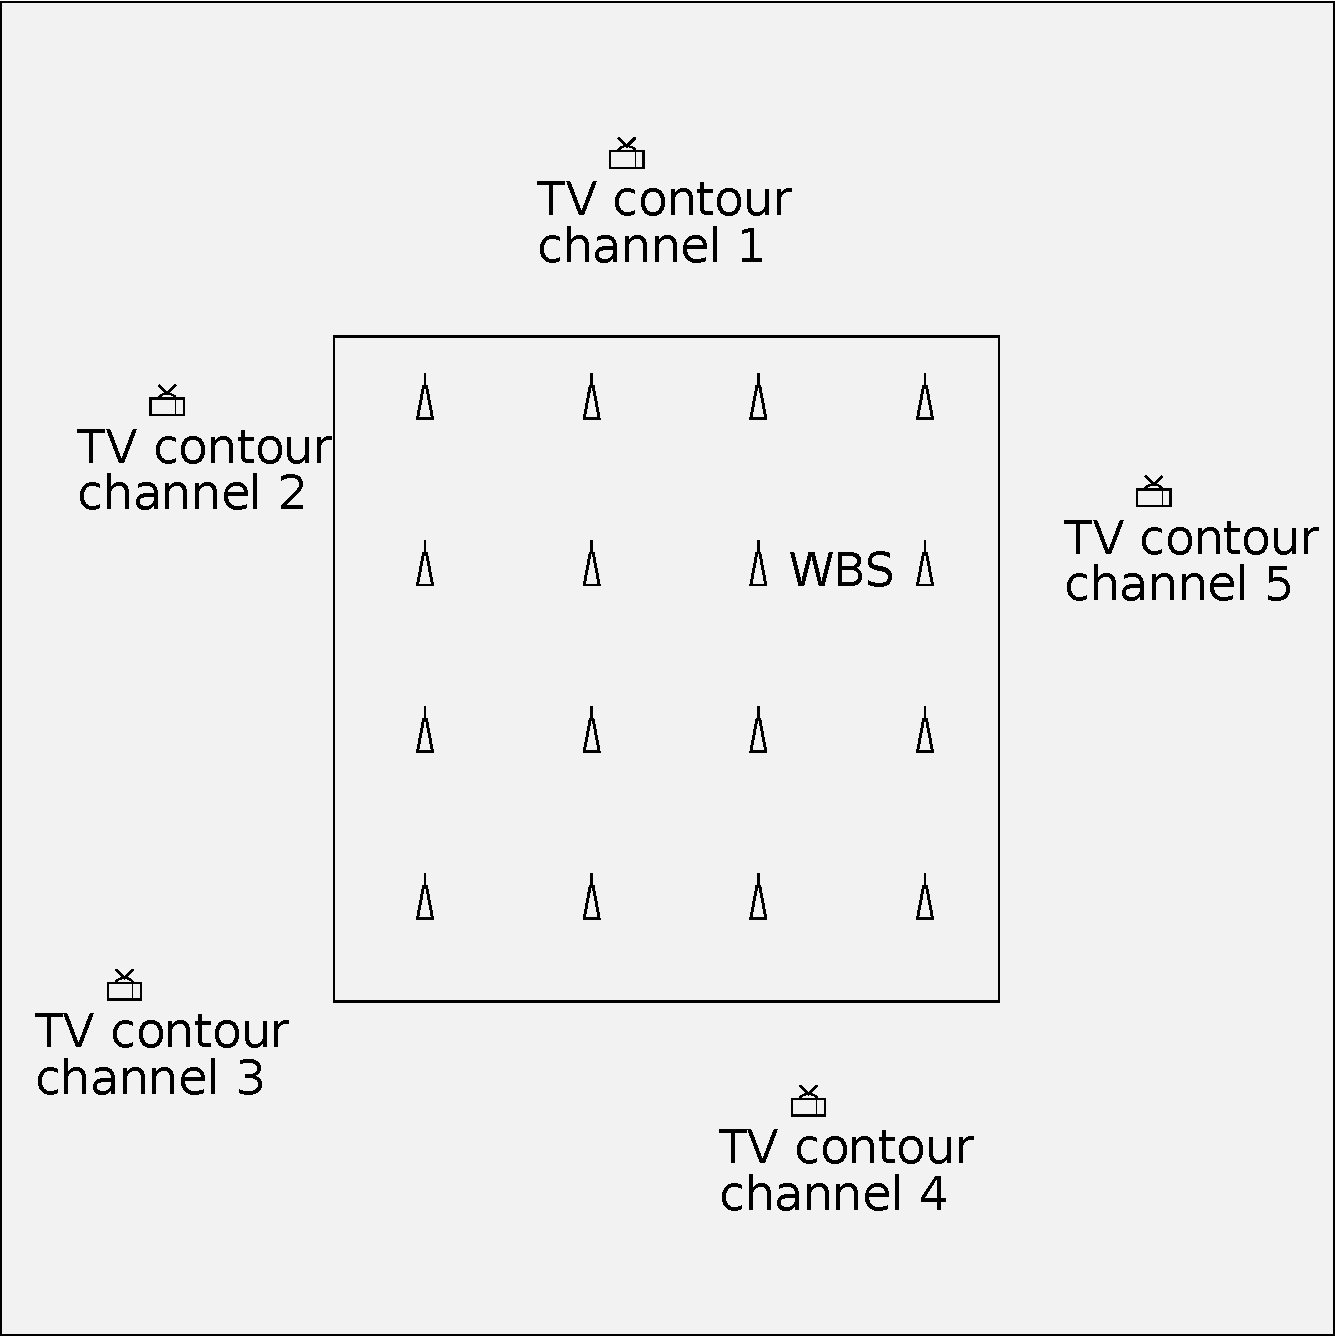
\includegraphics[width=0.5\linewidth]{layout.pdf}
  \caption{Layout of WBSs and TV contours}
  \label{sim:layout}
\end{figure}
The other parameters are listed in Table~\ref{6}ef{simulationparameter}. 

\begin{table}[!h]
\centering
\begin{tabular}{|l|r|}
  \hline
  Number of channels 						& 5 \\
  Number of WBSs							& 16\\
  Noise 									& $10^{-12}$W \\ % -90dbm
  Length of the square to locate WBSs		& 60km\\
  Distance between quasai terminal and WBS 	& 7km \\
  Interference threshold on TV contour 		& $10^{-7}$W \\ % -67dbm
  Path loss factor 							& 2 \\
  Standard deviation in flat shadowing		& 8\\
  Minimal WBS transmission power 			& 4W \\
  Maximal WBS transmission power 			& 40W \\
  Number of end terminals in network 		& 800 \\
  \hline
\end{tabular}
\caption{Simulation parameters}
\label{simulationparameter}
\end{table}

\subsection{Maximal Permitted Power Decision and the Distributed Channel Allocation Schemes}
In this section, firstly, we will evaluate which optimization in Section~\ref{powermap} is better to decide the maximal permitted transmission power, the adopted metrics are average power consumption, and SINR on end users.
Then with the decided better method, we will compare given the power map, how do the channel allocation schemes perform.
%Respectively with the power map obtained from linear programming and convex programming, we execute channel allocation problems.
We compare our proposed channel allocation scheme \textit{whiteCat} with three other distributed schemes, the random allocation scheme, whiteCase, No-regret learning and the centralized quadratic optimization introduced in Section~\ref{CA_fixedPower_2subproblem}, which is named as \textit{optimization}.


 \begin{figure}[h!]
    \centering
      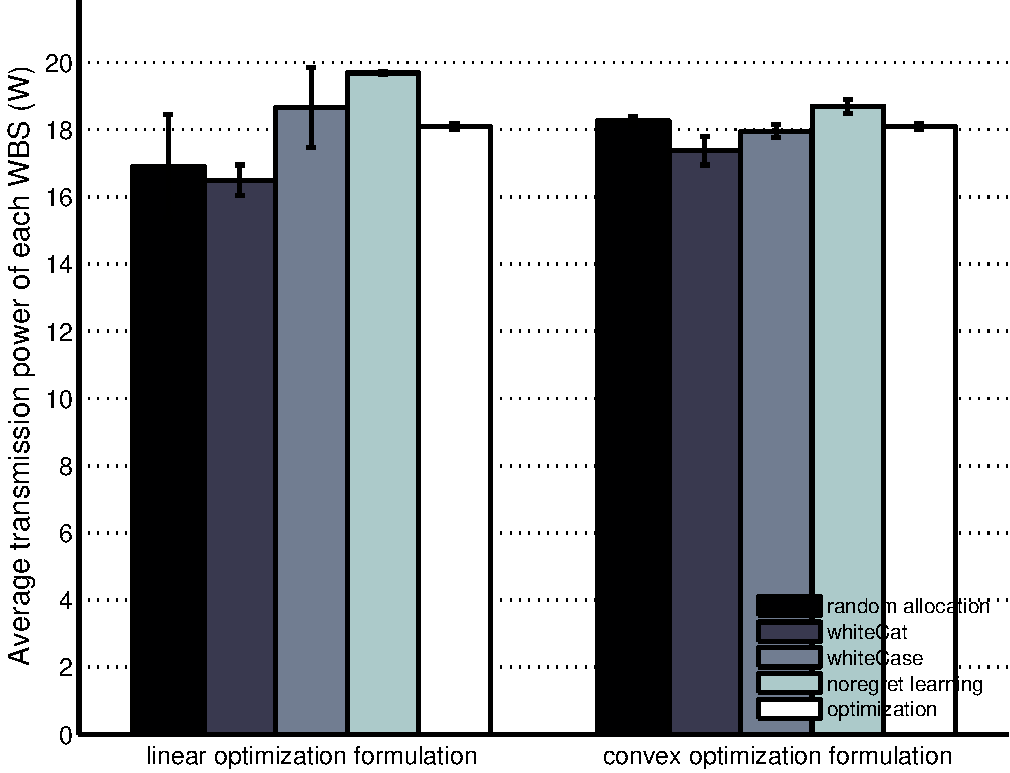
\includegraphics[width=0.8\linewidth]{3.pdf}
    \caption{Power consumed by different distributed spectrum allocation schemes under different ways deciding the maximal transmission power map}
\label{sim:group1_power}    
  \end{figure}
  
   \begin{figure}[h!]
       \centering
       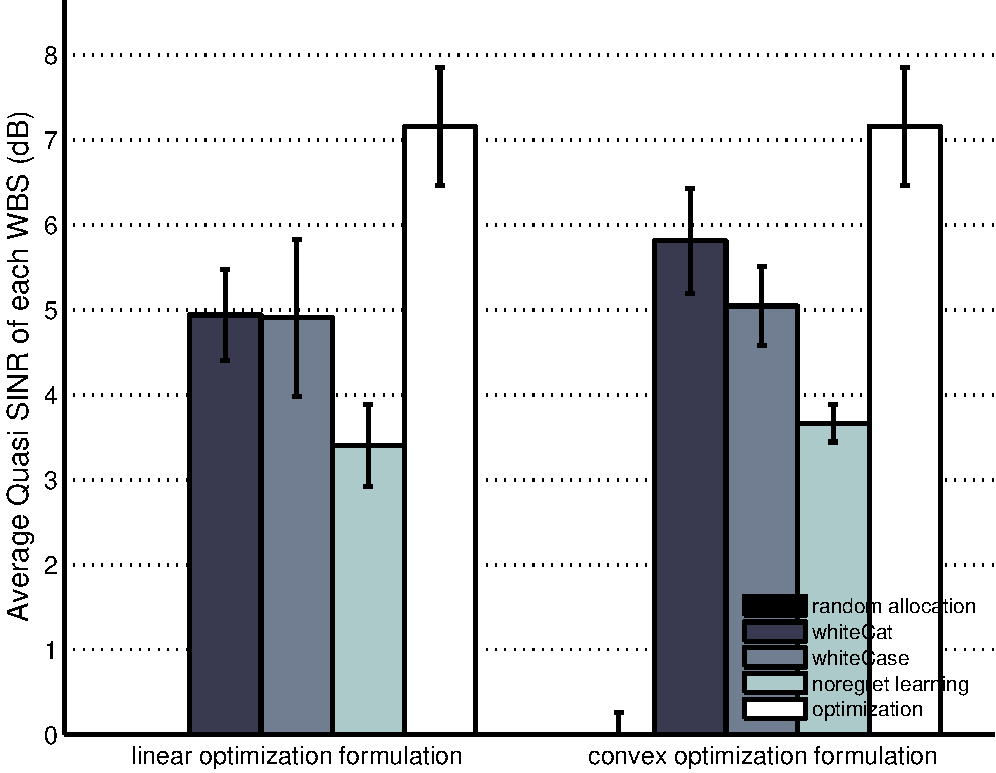
\includegraphics[width=0.8\linewidth]{4.pdf}
       \caption{QuasiSINR achieved by different distributed spectrum allocation schemes under different ways deciding the maximal transmission power map}
	\label{sim:group1_qsinr}       
     \end{figure}
  
 
  \begin{figure}[h!]
     \centering
     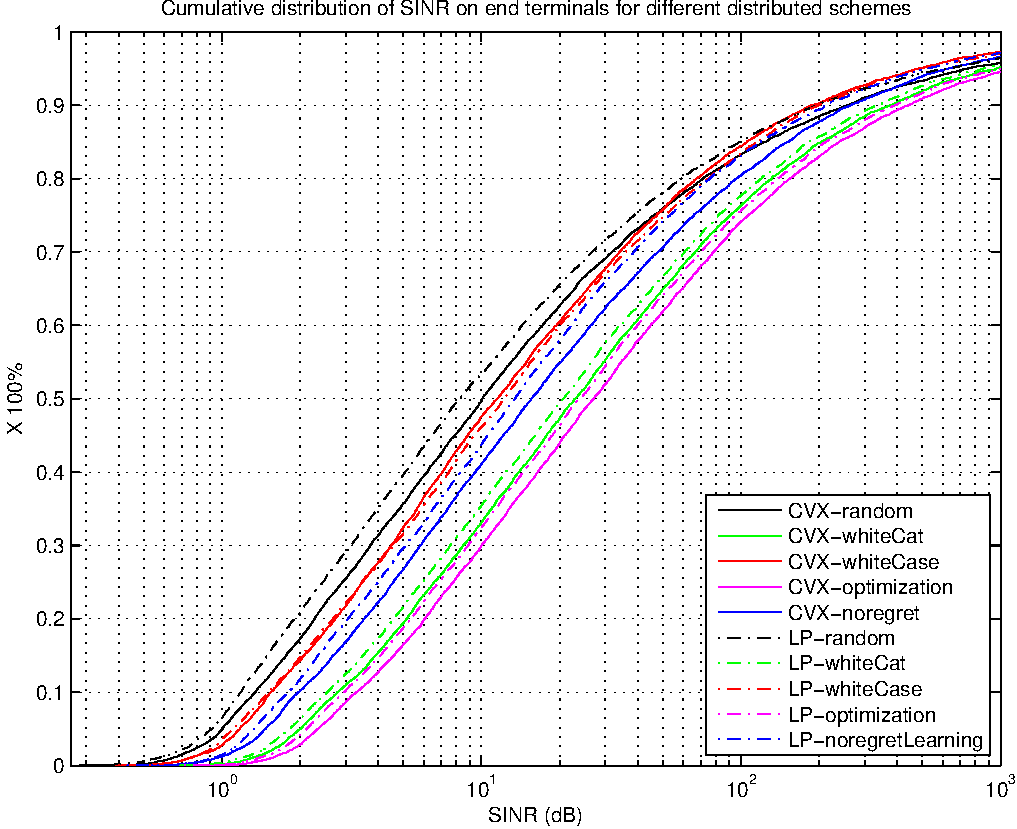
\includegraphics[width=0.8\linewidth]{5.pdf}
     \caption{CDF of SINR on end users obtained by different CA schemes under different methods to decide the maximal transmission power map}
\label{group1_sinr}     
   \end{figure}

\subsubsection*{Comparison of formulations to determine the maximal permitted power}
In section~\ref{powermap}, two different formulations are introduced to calculate the maximal permitted transmission power, \ie convex optimization and linear optimization respectively.
The convex optimization generates power levels which are with smaller difference compared with that obtained from linear optimization, which is shown in Fig.~\ref{lpcvx}.
In this section we will find out which formulation outperforms in terms of SINR on end terminals and transmission power consumption when distributed spectrum allocation schemes execute with the power maps.
%We simulate the 4 distributed spectrum allocation schemes with the  map obtained from , and then tell which maximal power map generation outperforms based on the performances of the 4 spectrum allocation schemes.
WBSs' locations are fixed whereas the location of TV contours, end terminals and the sequence for WBS to update are randomly decided.
In each run of simulation, end users select the WBS which brings it the best SINR performance.
Simulations are done for 100 times.
%we apply convex programming and linear programming to decide the maximal transmission power, and then the 4 distributed schemes are executed. 
Fig.~\ref{sim:group1_power} and~\ref{sim:group1_qsinr} show that when convex formulation is applied to decide the maximal power map, all the four distributed spectrum allocation schemes consume less transmission power consumption by 15\% to 30\% and achieve better QuasiSINR. 
The cumulative distribution function curve of SINR on end terminals is drawn in Figure \ref{group1_sinr}, where the x axis represents SINR level, and the y axis shows the cumulative proportion of end terminals whose SINR equals or smaller than that level. 
The curves show that except for the random method, all three other distributed schemes perform better in low SINR area (SINR $<10 dB$) with convex formulation, while worse in the high SINR area. 
Hence we adopt convex formulation to decide the maximal transmission power in the following simulation.


\subsubsection*{Comparison among channel allocation schemes }
After deciding the maximal permitted transmission power on each channel for each WBS, the data center distributes this maximal power map to all WBSs, and trigger the procedure of distributed channel allocation. 
\begin{figure}[h!]
  \centering
  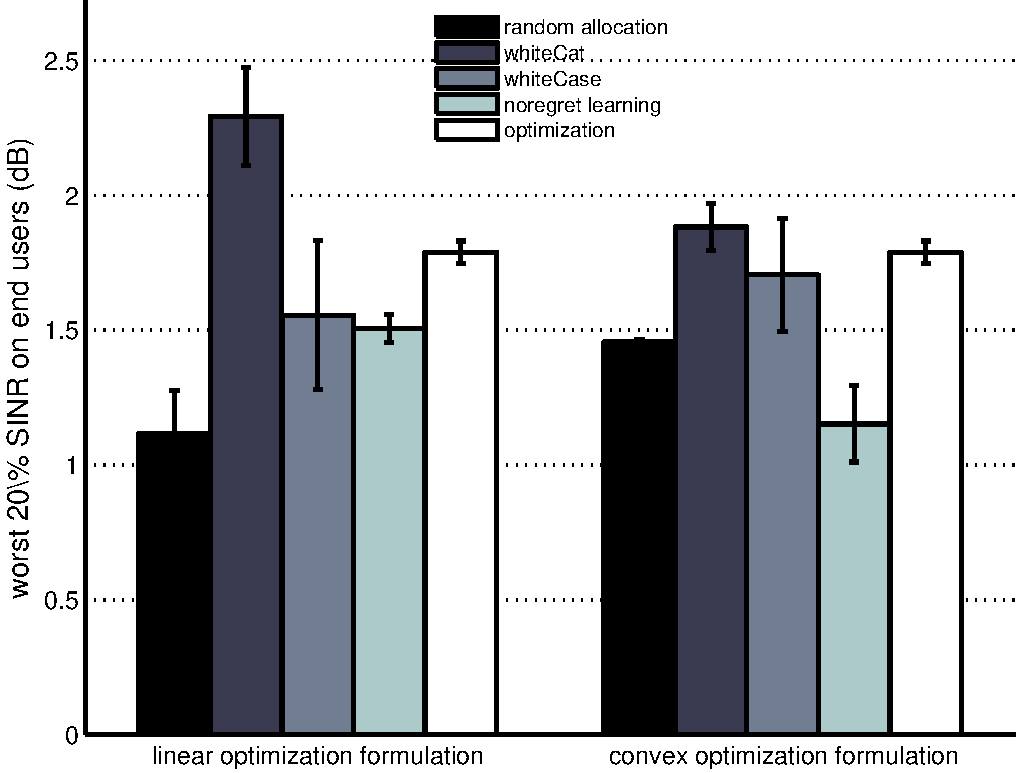
\includegraphics[width=0.8\linewidth]{1.pdf}
  \caption{The average SINR of the 20\% worst end terminals}
\label{group1_worst20sinr}
\end{figure}


The performance of the four spectrum allocation approaches working with the maximal power map calculated from convex formulation is elucidated in the right part of both Fig.~\ref{sim:group1_power} and \ref{sim:group1_qsinr}. 
We can see that WhiteCat consumes 12\% less transmission power than WhiteCase and No-regret learning schemes, whereas better QuasiSINR is obtained. 
The cumulative distribution function curve of SINR on end terminals with convex programming is presented in Fig.~\ref{group1_sinr} with dash lines, we can see that for any cumulative proportion under 90\%, the corresponding SINR level from Whitecat on end terminals is slightly (around 0.5-1 dB) but stably higher than that obtained by WhiteCase and No-regret schemes, and 3 dB higher than that in random scheme.

In each run of simulation, average value of the 20 \% end terminals with the worst SINR is recorded, and the averaged such value over 100 simulations is illustrated in Figure \ref{group1_worst20sinr} which shows WhiteCat achieves better performance for the worst suffered end terminals than WhiteCase and No-regret approaches.




\subsubsection*{Analysis on convergence process}

%Complexity: 
%For each player, there are at most $(n-1)*|\mathcal{C}|$ resources available for usage, while, because the produced congestion on each resource is independent on channel, in other words, the congestions involving the same pair of players are quantitatively identical, there are only $(n-1)$ quantitatively different congestions on one player's resources. So, the number of combinations with quantitatively non-identical congestions involved with that player is $2^{(n-1)}$, accordingly there are totally $n*2^{(n-1)}$ quantitatively different congestions for the whole the problem. We adopt the method of \cite{LectureA}, which resorts the congestions in a increasing sequence, and replaces the original congestions with integer values starting form 1. We call the integers as \textit{new} congestions. In this way the preferences of the players are preserved and we can find easily the biggest possible congestion is $n*2^{(n-1)}$, which is the upper bound for the number of steps towards convergence.
In the congestion game, each player has at most $(n-1)*|\mathcal{C}|$ resources available for usage, so there is no polynomial steps converging to NE, while, simulation shows the algorithm can quickly converge to NE when the number of WBS is up to 100. 
%Figure \ref{100converge} shows that for 100 WBSs, whitecat executes at most 5 iterations (in one iteration all WBSs update their choices). 
Figure \ref{convergeComp} depicts one instance of simulation, where WhiteCat converges quickly, No-regret produces oscillation but converges finally, while WhiteCase can not converge thus has to be enforced stop after 16000 updates. %\todo{replot}%, whereas 

%\begin{figure}[h!]
%\label{100converge}
%  \centering
%  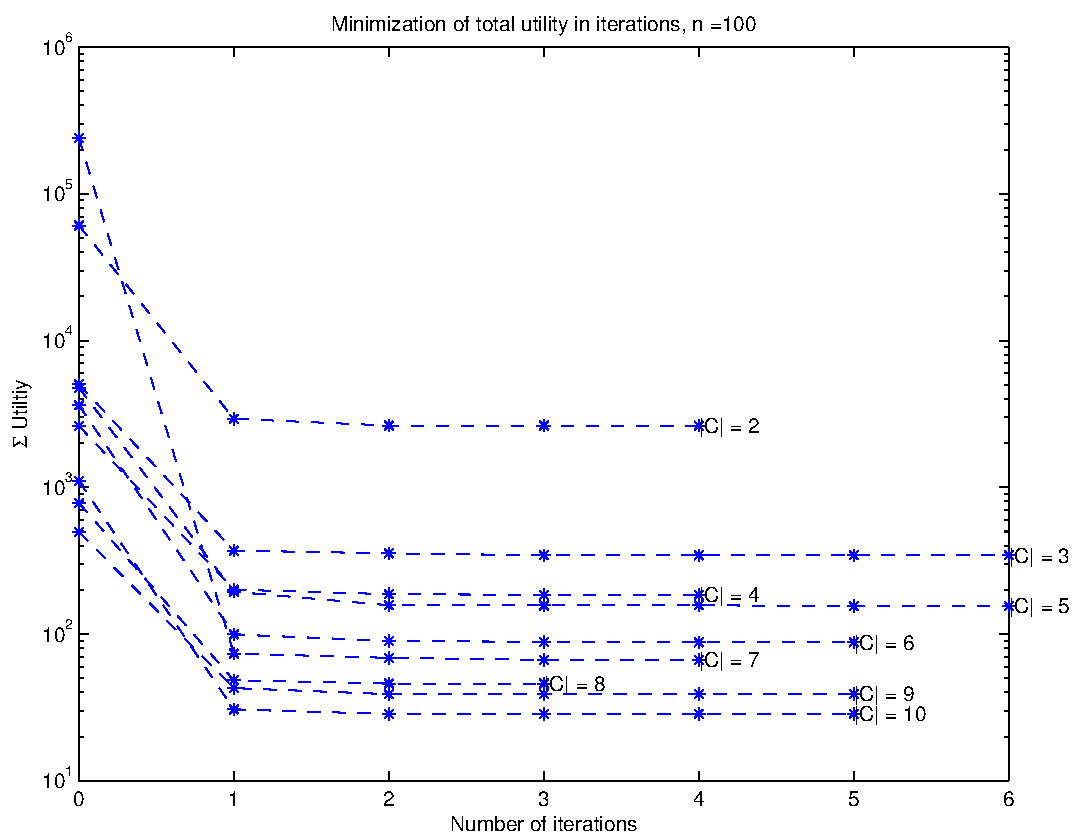
\includegraphics[width=0.65\linewidth]{CAConverenge100.pdf}
%  \caption{100 WBSs, 2-10 channels}
%\end{figure}


\begin{figure}[h!]
  \centering
  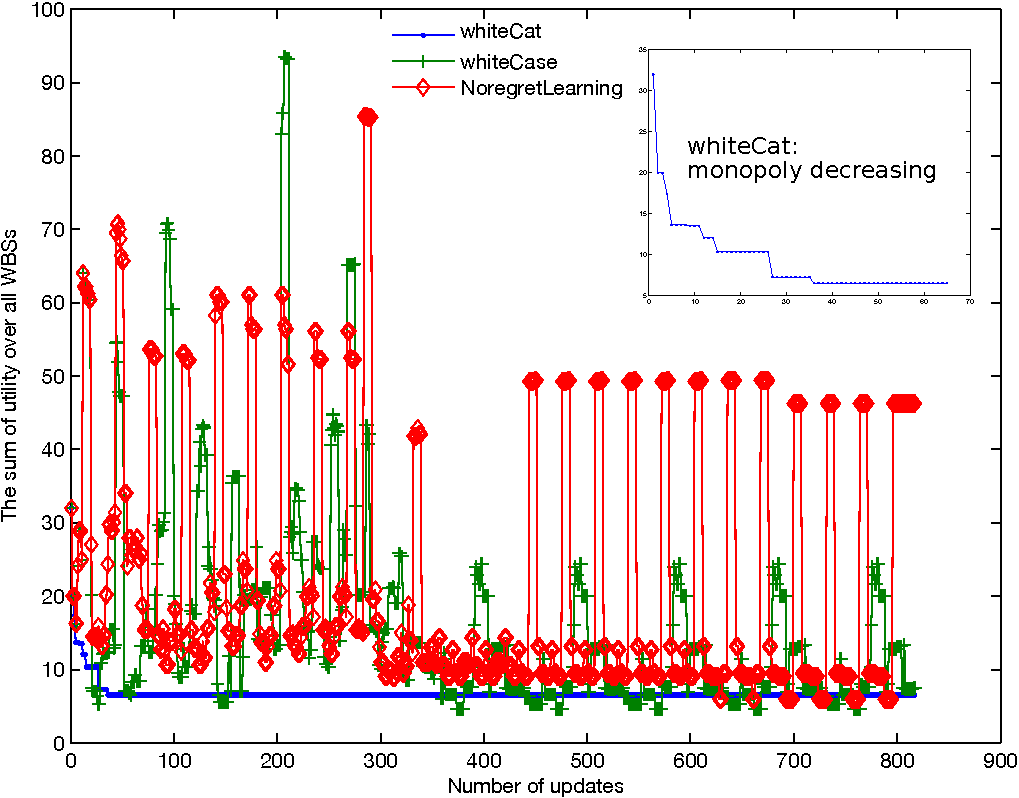
\includegraphics[width=0.8\linewidth]{30_31.pdf}
  \caption{Convergence with three different schemes in one simulation instance}
\label{convergeComp}
\end{figure}


We also compare the convergence speed between WhteCat with no-regret scheme. We fix 16 WBSs' location working with 4 channels, whereas the location of TV contours and end terminals are randomly decided. We account each WBS accessing the base station (refer to \ref{whitecat}) as \textit{one step}. We record the number steps before convergence. Table \ref{convergencespeed} illustrated the average number of steps needed for convergence in 100 runs of simulations. As there is no guarantee for WhiteCase to converge, we stop the channel allocation process after 16000 steps (1000 rounds). We can see WhiteCat is 20 times faster than no-regret, and the relatively small confidence interval shows that WhiteCat's convergence is not affected obviously by different network conditions, which is reasonable as more knowledge of the network is known by users executing Whitecat. As to average running time for each convergence with Matlab, Whitecat is much smaller than the other two schemes, as the nonlinear solver LINDO to be discussed in next subsection, the running time is about 40 minutes. Figure \ref{convergeComp} reflects one instance of the convergence of three schemes in one run of simulation. Notice that there is a slight rise when the value on the X-axis is 35, which comes from the difference between \ref{compare} and \ref{allPotential}.

\begin{table}[!h]
\centering
\begin{tabular}{|l|c|c|c|}
  \hline
  Scheme			 						& average \#steps 	 		& 95\% CI			&average time (s)\\
    \hline
  whitecat									& 58											& 5.6						&2\\\hline
  whitecase 								& 4587 											& 2742						&50\\\hline % -90dbm
  non regret									& 1916											& 1541						&144\\\hline
  potential game 							& 120							& 10										&4\\
  \hline
\end{tabular}
\caption{Convergence speed of the distributed channel allocation schemes}
\label{convergencespeed}
\end{table}


\subsubsection*{Stability of SINR in the process of channel allocation}
WBS provides service to end users in the process of channel allocation. 
A certain SINR corresponds to certain transmission configurations like modulation type and data rate. Oscillation of SINR may cause reconfiguration, reduced throughput or delay variance, thus is not preferred. We propose a metric \textit{Cost of Oscillation} (\gls{COS}) to represent the stability of SINR in the converging process. We assume each update step takes the same amount of time which is 1 time unit, the variance of SINR on end user $i$ at time point $t+1$ compared with that at time $t$ is $\varDelta  \gamma_i(t+1)=\mid\frac{\gamma_i(t+1)-\gamma_i(t)}{\gamma_i(t)} \mid$. The COS value for one network applied with a certain channel allocation scheme is,
\begin{equation}
\label{cos}
			COS = \sum\limits_{t=1}^T   \sum\limits_{i\in \mathcal{N}} \varDelta  \gamma_i(t)
			\end{equation}
$\gamma_i(0)$ is the SINR for $i$ before starting channel allocation. The variance of SINR in channel allocation process is shown in table \ref{costable} from which we can see WhiteCat achieves only 6\% of oscillation on SINR compared with No-regret approach.
\begin{table}[!h]
\centering
\begin{tabular}{|l|c|c|}
  \hline
  Scheme			 						& COS 					& 95\% Confidence interval\\
    \hline
  Whitecat									& 8850					& 2984\\
  Whitecase 								& 246790 				& 168050\\ % -90dbm
  No-regret									& 145460				& 1541\\
  \hline
\end{tabular}
\caption{Variance of SINR during the converging phase}
\label{costable}
\end{table}
%\todo{Switching to a different channel also brings cost on time and perfomance, tbc}



\subsection{Performance of joint power and channel allocation: cascaded distributed schemes vs. joint distributed/centralized schemes}
As introduced in section~\ref{powerAllocation}, after channel allocation is conducted, transmission power will be adjusted in a distributed manner. 
In other words, power and channel allocation is completed by executing two sequential distributed schemes.
%Distributed channel allocation schemes, along with the power adjustment, are compared with two other schems.
As comparisons, we implement two joint power channel allocation schemes.
One is centralized optimization introduced in section~\ref{opt_channelAndPower}, which is used as upper bound in the comparison.
The other comparison is distributed joint power and channel allocation scheme~\cite{pimrc_2012} which is introduced in section~\ref{relatedWork}.
We need to point it out that, scheme proposed in~\cite{pimrc_2012} doesn't aim to improve the SINR on end terminals, but on the sum of produced and received interferences.

The performance of joint channel and power allocation schemes are presented in Fig.~\ref{CAPA_utility}, \ref{CAPA_power} and \ref{CAPA_quasiSINR} in terms of total utility, power consumption and achieved quasiSINR respectively.

In Fig.~\ref{CAPA_utility}, we can see that together with the distributed power allocation method, DiCAPS achieves similar utility with the centralized channel allocation optimization, and the utility is close to the centralized joint channel and power allocation
This means that DiCAPS approaches the upper bound in terms of total utility.
Fig.~\ref{CAPA_power} shows DiCAPS together with power allocation consumes the least power.
Fig.~\ref{CAPA_quasiSINR} demonstrates the cumulative distribution of SINR on all end terminals,
.

\begin{figure}[h!]
  \centering
  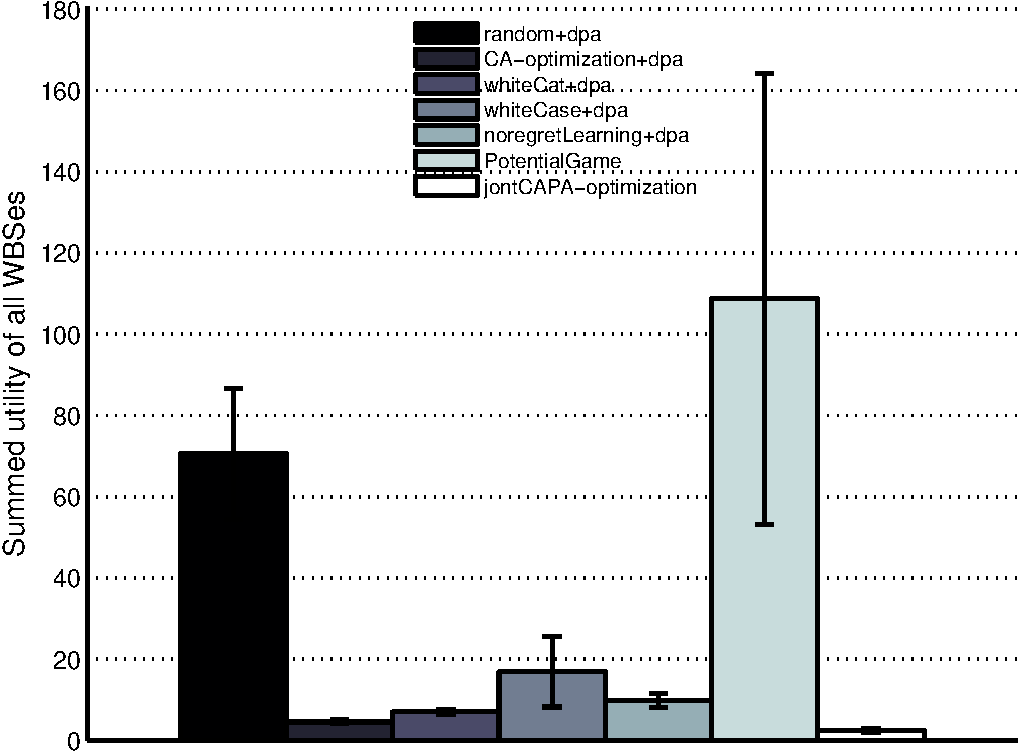
\includegraphics[width=0.8\linewidth]{16.pdf}
  \caption{Summed utility of all WBSs, which is the objective in problem~\ref{problem}. dpa in legend represents \textit{distributed power allocation}}
\label{CAPA_utility}
\end{figure}
%{ \label{summedU:sub2}	  


%\begin{figure}[h!]
%  \centering
%	\subfigure[After channel allocation]{	  \label{summedU:sub1}	  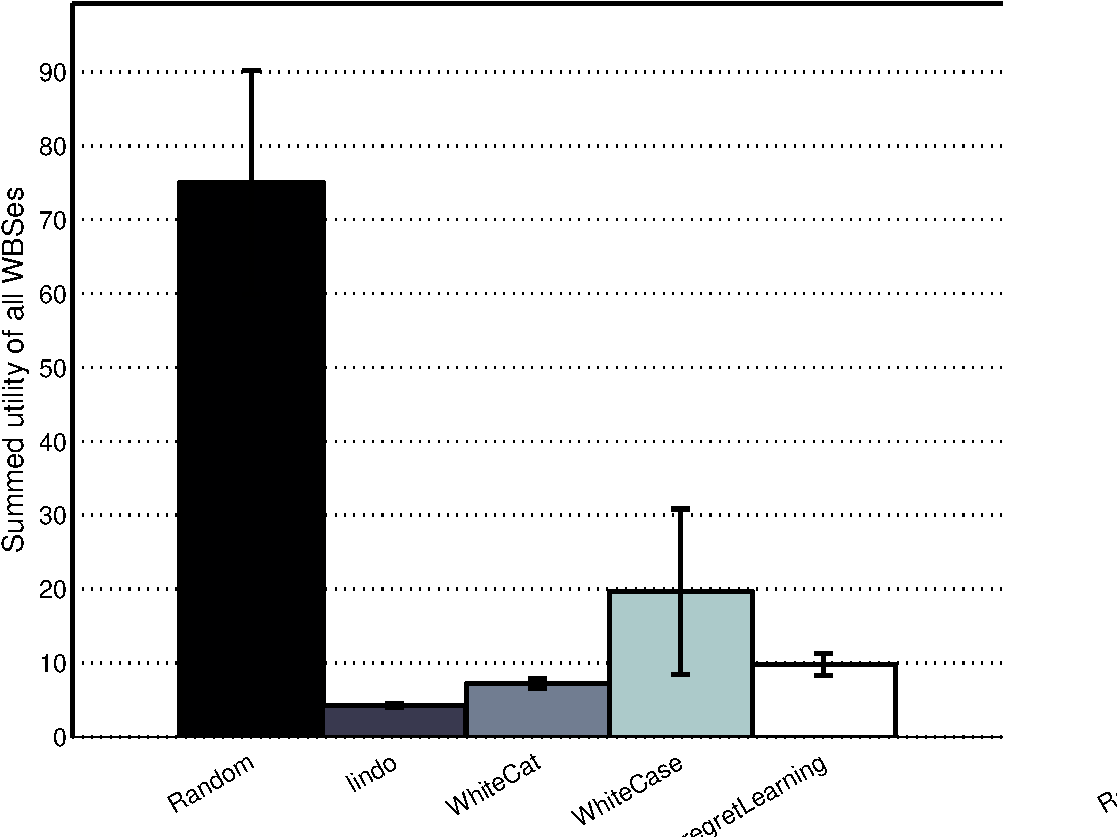
\includegraphics[width=0.47\linewidth]{12.pdf}}
%	\subfigure[After channel and power allocation]{  \label{summedU:sub2}	  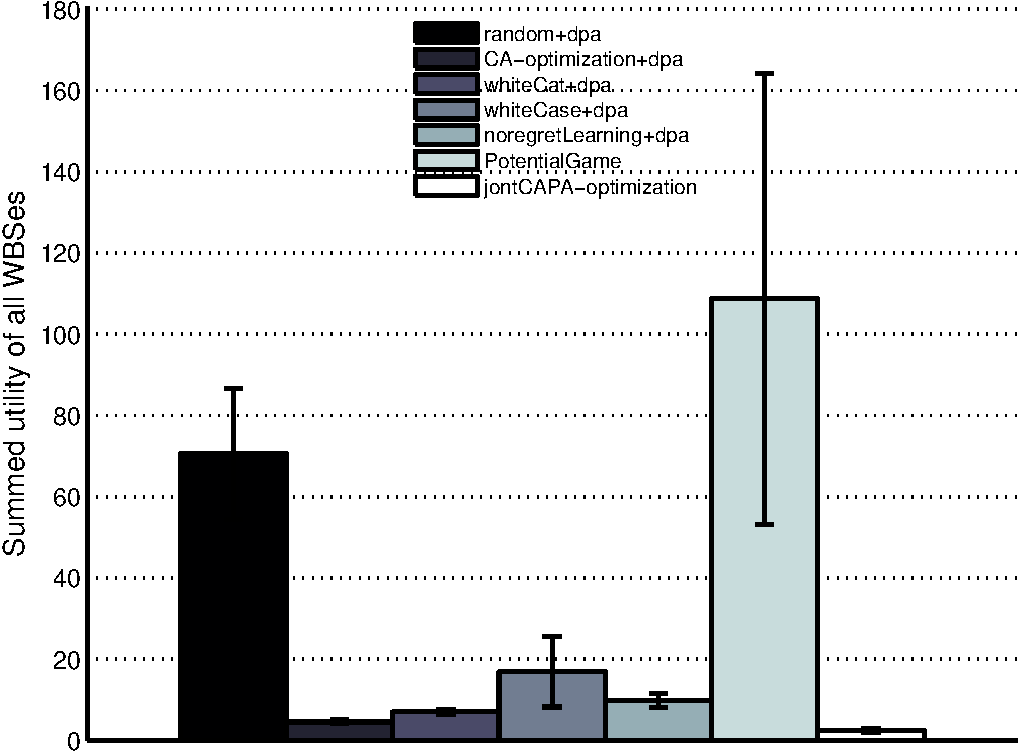
\includegraphics[width=0.47\linewidth]{16.pdf}}
%  \caption{summed utility of all WBSs, which is the objective in problem~\ref{opt}f{opt}}
%  \label{utility}
%\end{figure}



\begin{figure}[h!]
  \centering
  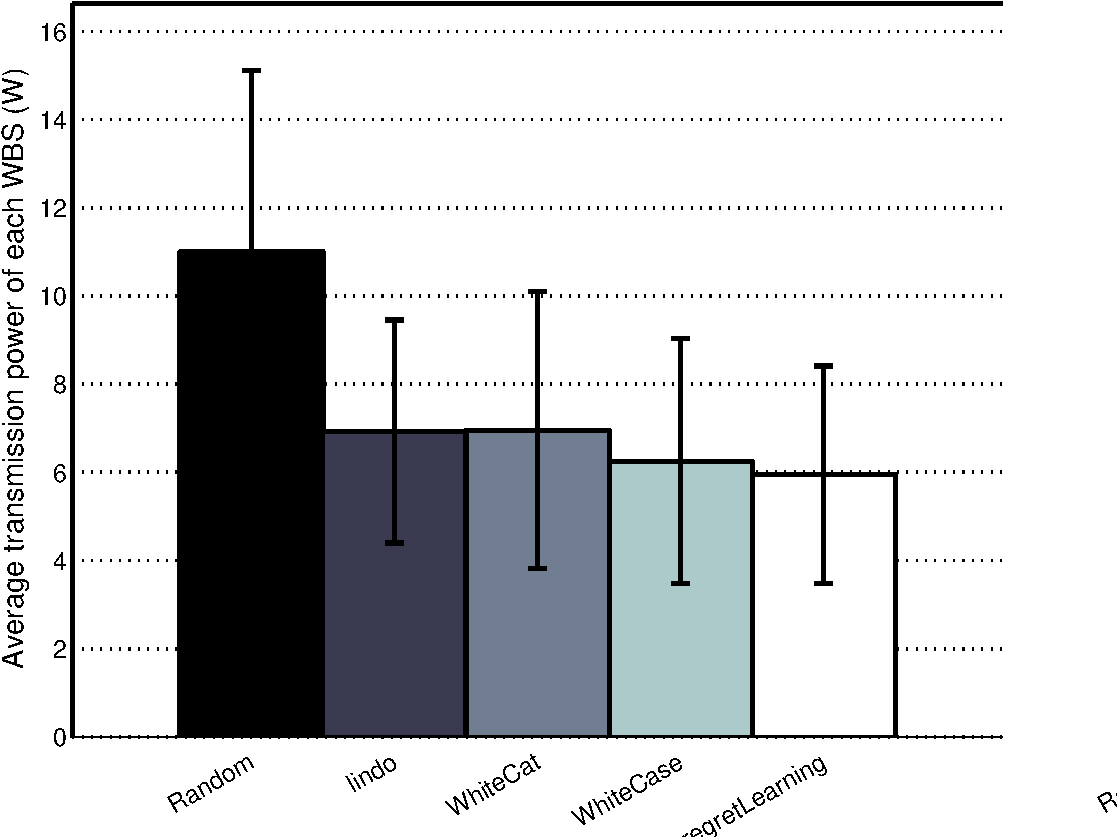
\includegraphics[width=0.8\linewidth]{14.pdf}
  \caption{Average transmission power of one WBSs}
\label{CAPA_power}
\end{figure}

%\begin{figure}[h!]
%  \centering
%  	\subfigure[After channel allocation]{\label{power:sub1}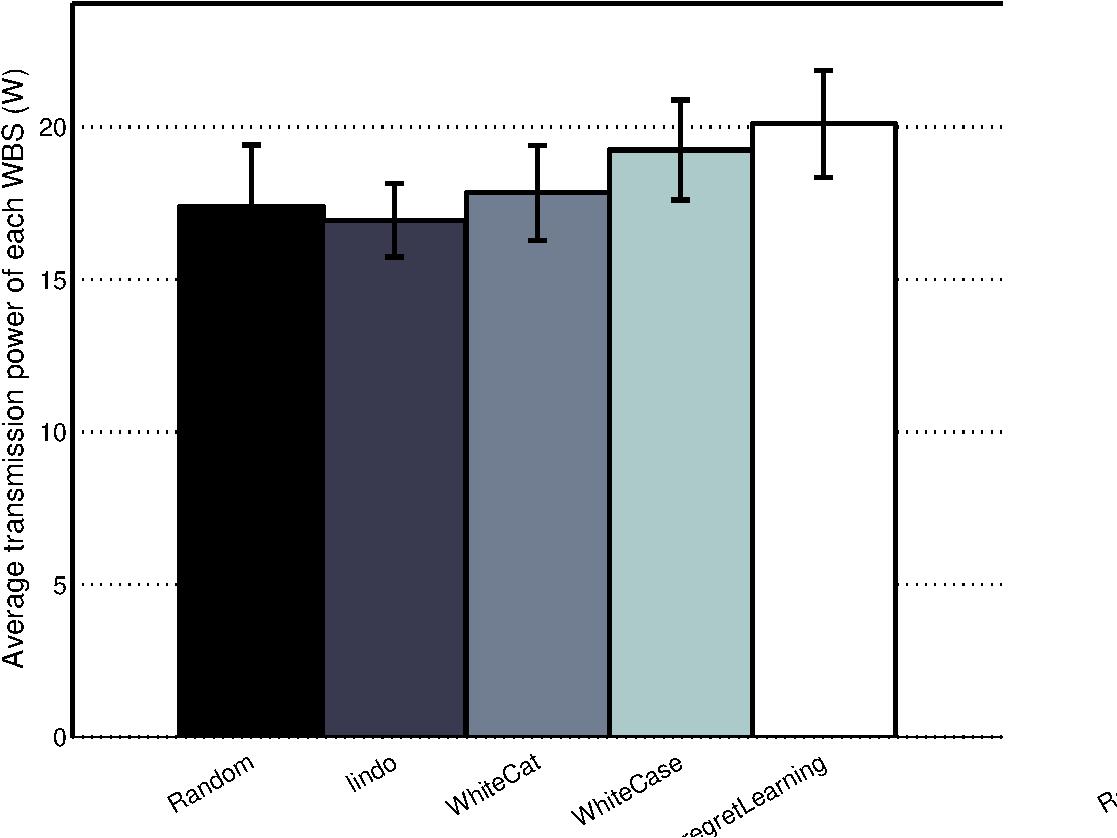
\includegraphics[width=0.47\linewidth]{10.pdf}}
%  	\subfigure[After channel and power allocation]{\label{power:sub2}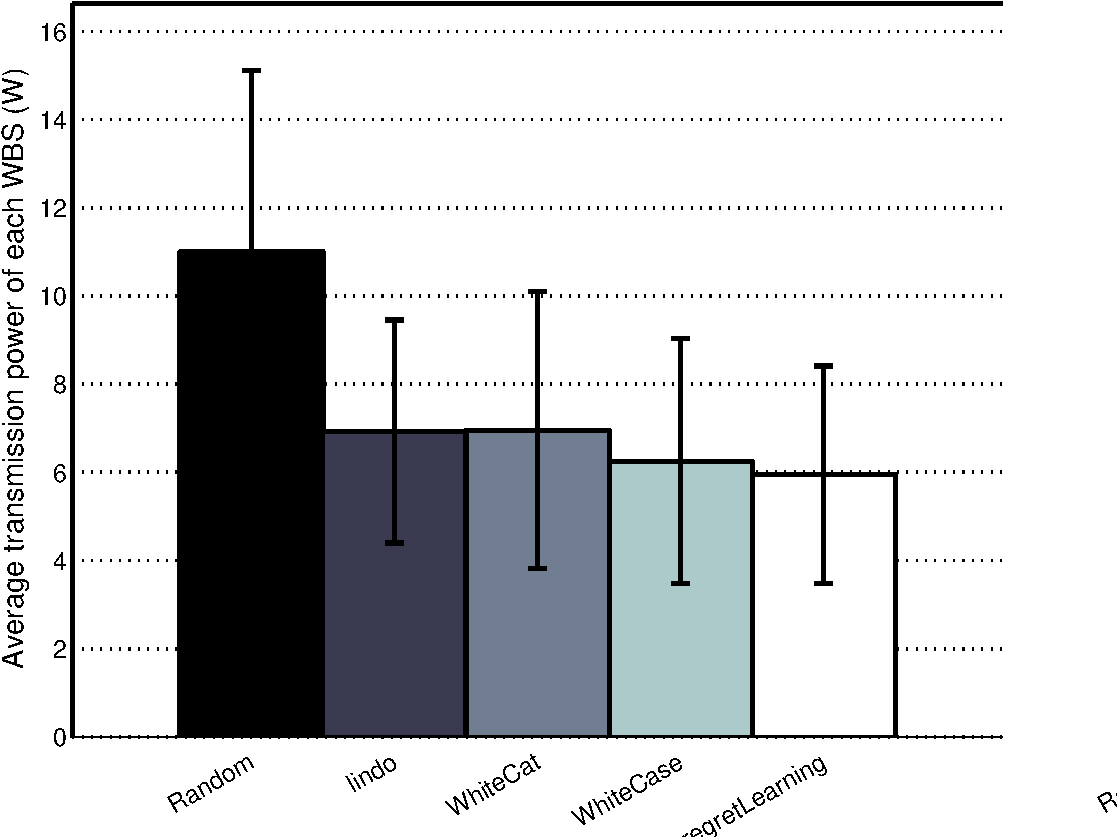
\includegraphics[width=0.47\linewidth]{14.pdf}}  	
%  \caption{Average transmission power of one WBSs}
%  \label{power}
%\end{figure}

\begin{figure}[h!]
  \centering
  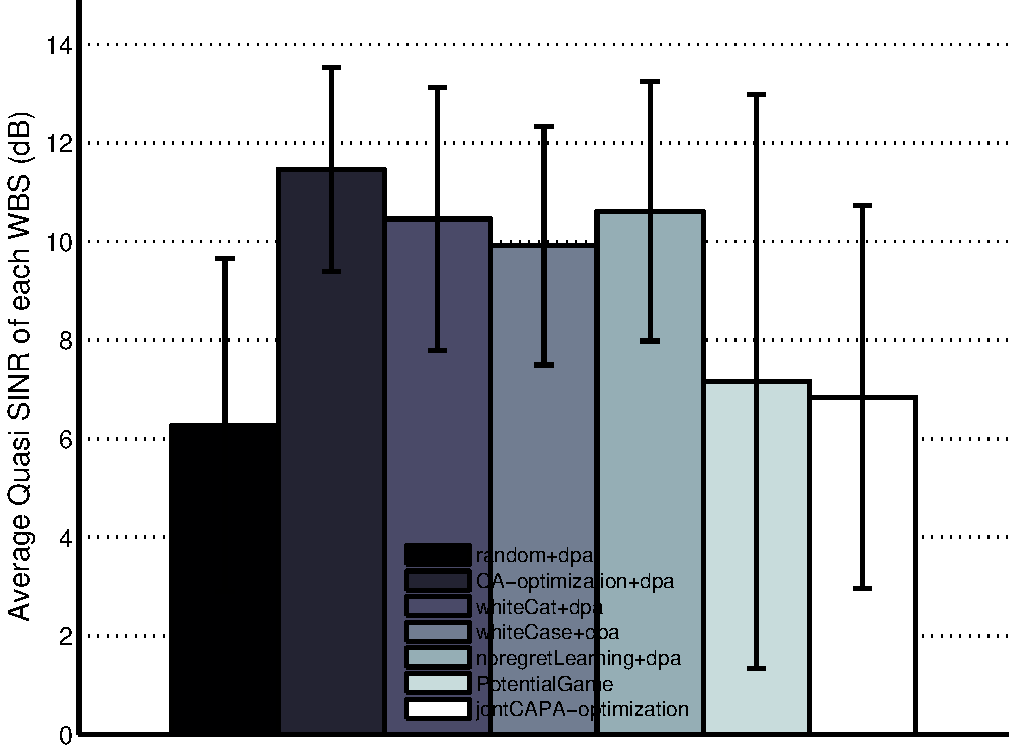
\includegraphics[width=0.8\linewidth]{15.pdf}
  \caption{Average quasiSINR of a WBS}
\label{CAPA_quasiSINR}
\end{figure}


%Compare the two figures in Figure \ref{utility}, \ref{power},\ref{quasiSINR}, we can see that transmission power is reduced by 50\% to 70\% for all schemes except for the random selection scheme, and the utility and quasiSINR are almost the same.




%\subsection{Comparison between distributed and centralized scheme  }

%After comparing the performances of WhiteCat with the other two heuristic solutions, we have a look at the difference between these distributed approaches with the centralized optimization method. For these heuristic schemes, the sequence to update influences the final performance, while, it is very difficult to find out the optimal sequence which achieve the best performance, for our simulation configuration, the number of different sequence for 16 WBSs is $16!$ which has order of magnitude of 14. For demonstration purpose, we choose 100 different update sequences randomly for 100 times of simulation. In each simulation the sequence of WBS to update their channels is randomly decided be identical for all the 4 schemes. As solution of optimization has nothing to do with sequence, we only solve the optimization problem for once. We fixed the location of WBSs and PU contours, only leave the end terminals randomly scattered in the inner square area in each simulation. 

%Figure \ref{perf1} reflects the performance of power consumption, QuasiSINR, and standard deviation of QuasiSINR when we apply the different schemes to the network. The upper left subplot illustrates that Whitecat consumes the least power compared with the other heuristic schemes along with the centralized optimization scheme. Upper right subplot shows that whitecat can achieve better QuasiSINR than Whitecase and non-regret approaches, but about 10 \% worse than the solution obtained from LINDO. Unsurprisingly, randomly choosing channels leads to the worst performance on QuasiSINR. The subplot below depicts the standard deviation of QuasiSINR from the five schemes, we can see the standard deviation of QuasiSINR achieved by whitecat is bigger than whitecase, non-regret and centralized optimization, which can be explained by Figure \ref{cdf}. 

%Fig.~\ref{powerQuasiSINR} shows the average power consumption and average QuasiSINR over all WBSs and rounds of simulations. 
%WhiteCat consumes the least of power except for the random scheme. while, Lindo outperform others 
%\begin{figure}[h!]
%  \centering
%  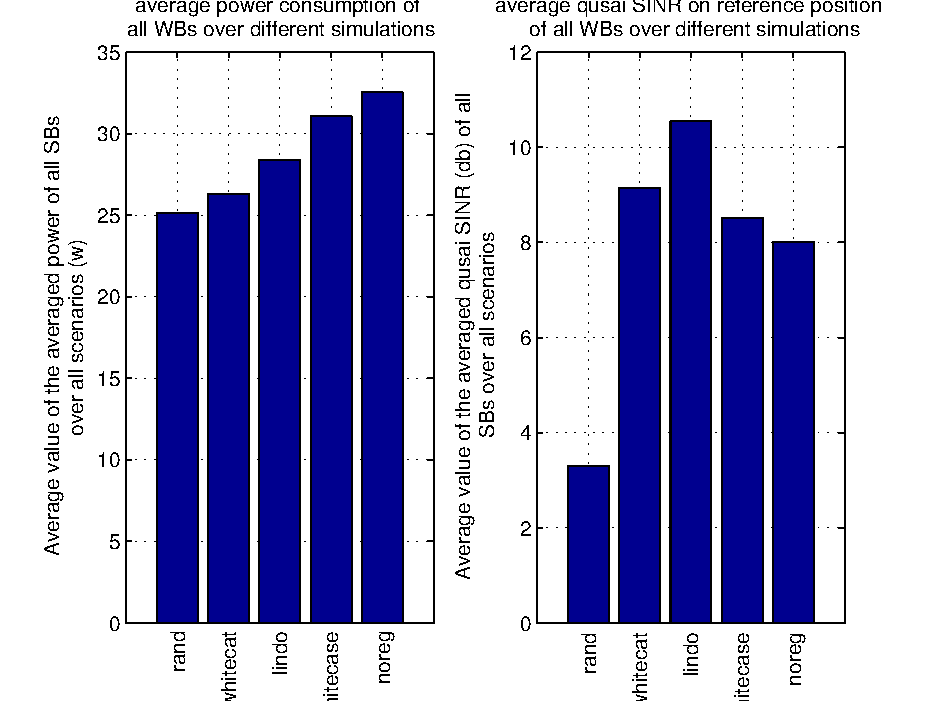
\includegraphics[width=1\linewidth]{powerQuasiSINR.pdf}
%  \caption{Average Power consumption and QuasiSINR}
%\label{powerQuasiSINR}
%\end{figure}

%Fig.~\ref{joint_SINRcdf} demonstrates the cumulative distribution of SINR on all end terminals, where the centralized optimization achieves 3 dB better SINR on end terminals than distributed schemes, which means there is still big space to improve the performance of decentralized approaches.

%\begin{figure}[h!]
%  \centering
%  	\subfigure[After channel allocation]{\label{fig:sub1}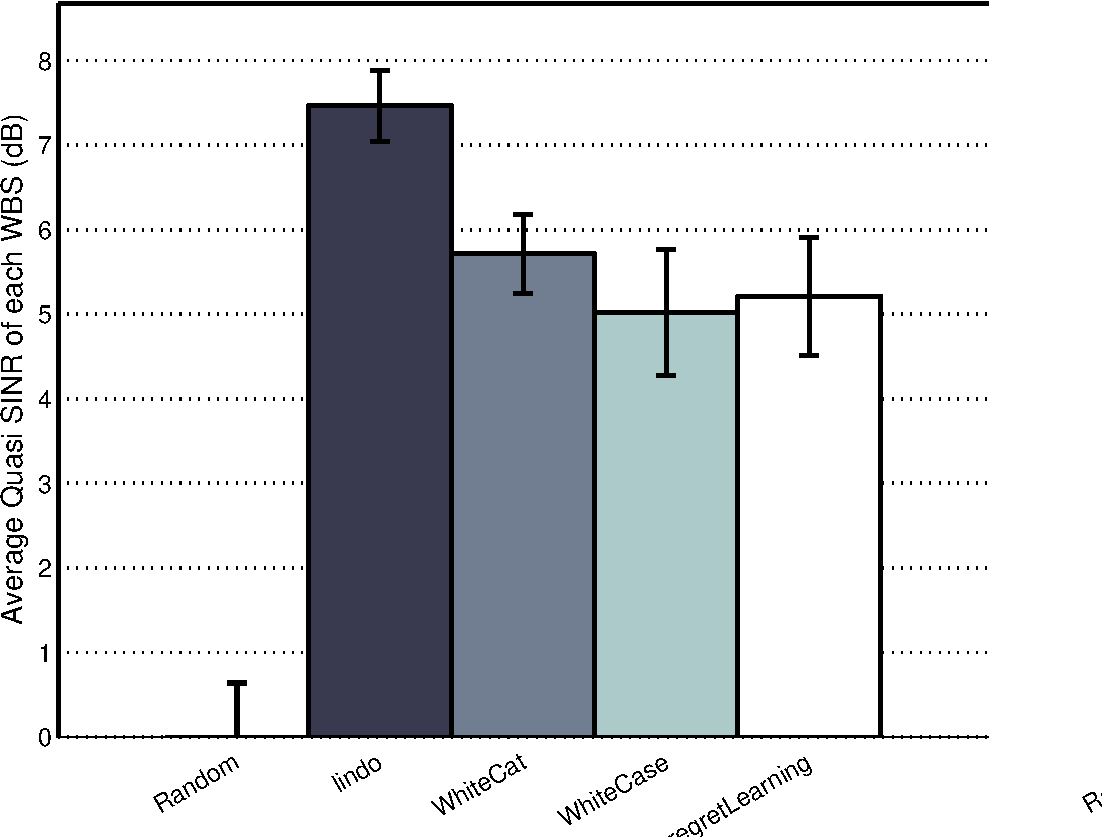
\includegraphics[width=0.47\linewidth]{11.pdf}}
%  	\subfigure[After channel and power allocation]{\label{fig:sub2}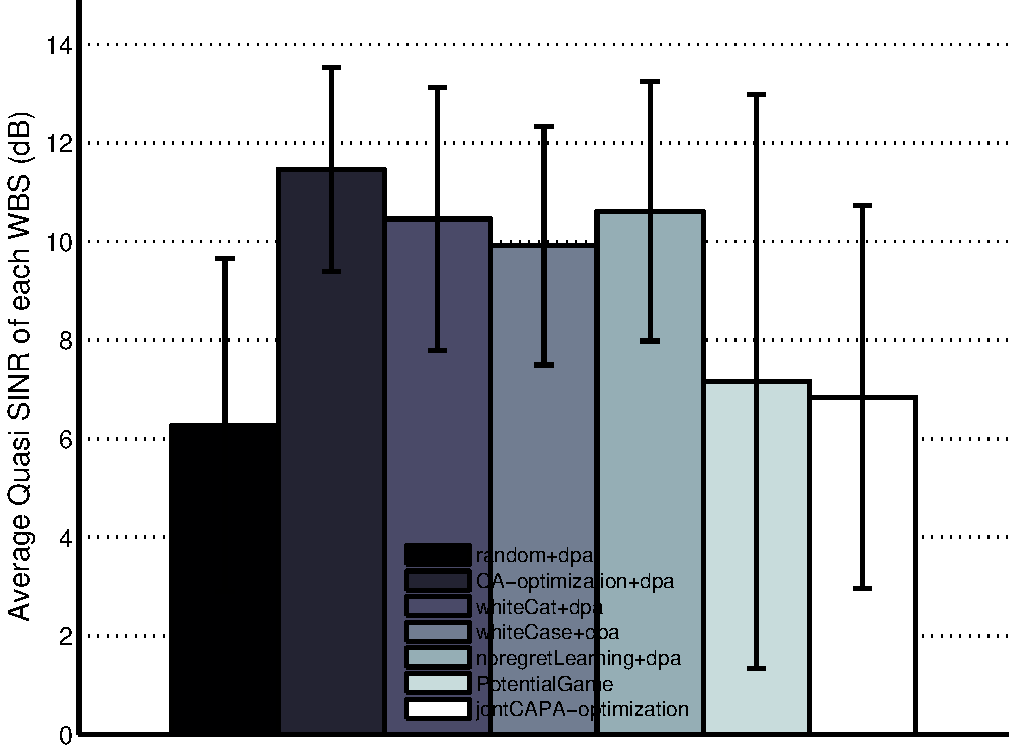
\includegraphics[width=0.47\linewidth]{15.pdf}}  	
%	  \caption{quasiSINR: SINR at the reference point}
%	  \label{quasiSINR}
%\end{figure}

%\begin{figure}[h!]
%  \centering
%      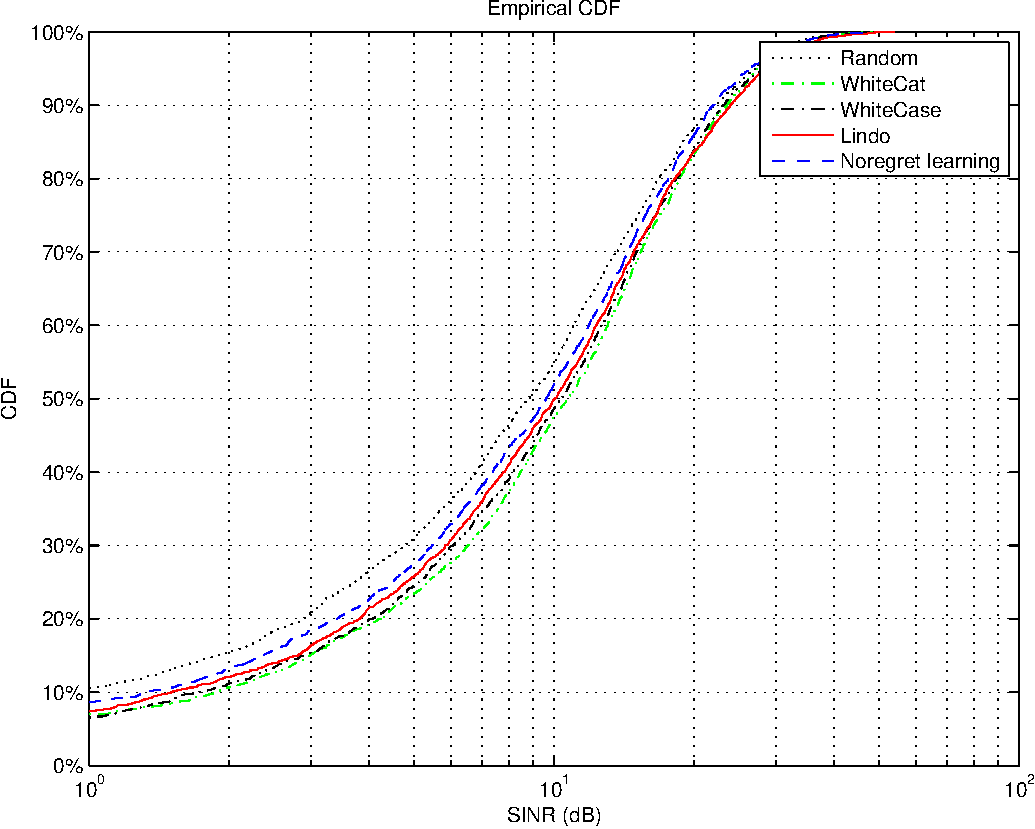
\includegraphics[width=0.9\textwidth]{20.pdf}
%  \caption{SINR on end users after channel allocation}
%\end{figure}

\begin{figure}[h!]
  \centering
  \label{joint_SINRcdf}
      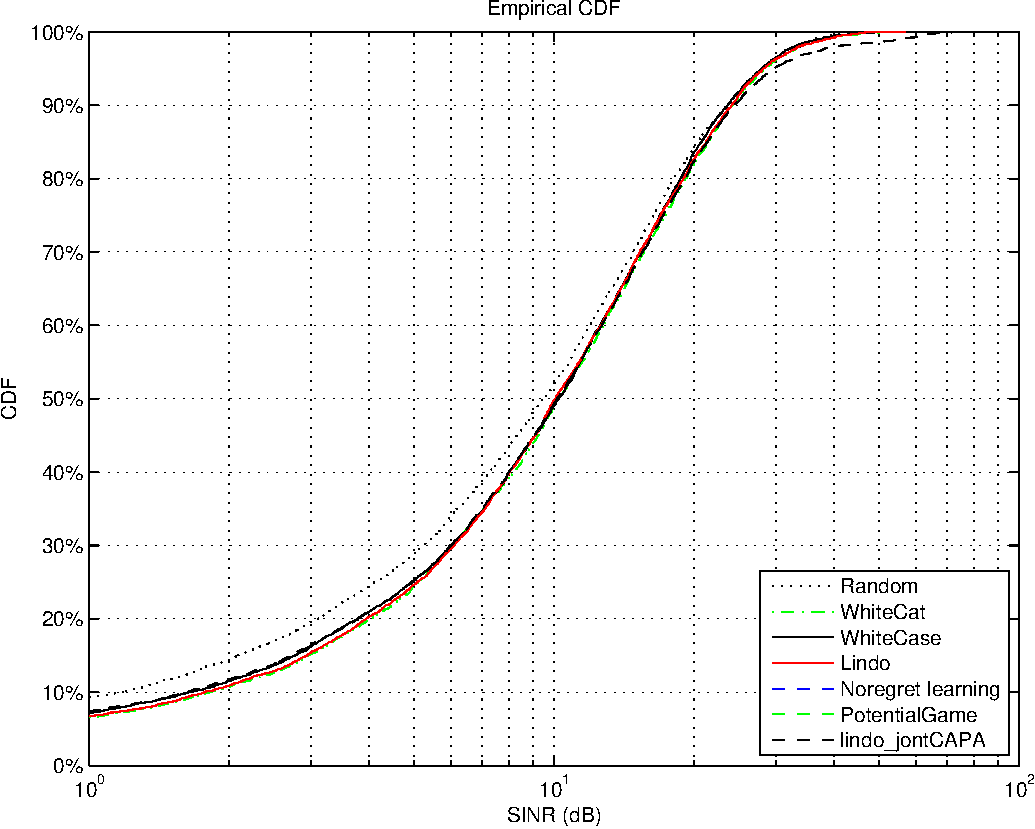
\includegraphics[width=0.9\textwidth]{24.pdf}
  \caption{SINR on end users after channel and power allocation}
\end{figure}

\section{Conclusion}
We propose a method to assign maximum transmission power to secondary users to make full use of the white TV spectrum. The second contribution of this chapter is the design of a distributed channel assignment scheme called WhiteCat which is designed for secondary users to decide which chunk of spectrum should be used in order to improve cell performance in the down-link transmission direction. WhiteCat provides end terminals better SINR with less transmission power, and converges to one pure Nash equilibrium in a faster speed compared with two other schemes (greedy best response as well as a no-regret learning scheme). WhiteCat is formulated into a standard congestion game which proves the convergence of the scheme. WhiteCat requires a central data base containing information about the previously allocated channels to secondary users as well as their positions and propagation information among the base stations. Compared to previous work that suggests the use of a central data base for base station registration and channel validation, this is a minor overhead to be introduced. 
For future work we will address the problem of allowing base stations to set the transmit power arbitrarily within the maximum transmit power limit. 

\backmatter
\begin{appendices}
%\appendix
%\addcontentsline{toc}{section}{Appendix~\ref{noconvergence}: Proof of Theorem \ref{noconvergence}}
\chapter{Proof of Theorem \ref{noconvergence}}
\label{proof}

For selfish best response approach, the utility function is set as follows,
	\begin{equation}
\label{selfishutility}
		u_i=\frac{\sum_{c(i)=c(i)} \tilde{f_{ji}}+N_0}{P_i\cdot h_{ii}}
	\end{equation}

\begin{proof}

In order to simplify the proof, we assume $N_0=0$.
Consider one WBS $i$ executing algorithm \ref{whitecatalgo} with utility \ref{selfishutility}, and updates its channel from $c_i$ to $c_i'$, we denote $u_k', k\in \mathcal{N}$ as the utility of WBS $k$ when $i$ chooses channel $c_i'$, accordingly, the summation of utilities of all WBSs after $i$ changing to $c_i'$ is $U'=\sum_{\forall k\in \mathcal{N}, c(i)=c_i'}u_k'$.
\begin{equation}
\label{xxx}
\begin{split}	
U'
& =u_i' + \sum\limits_{j\in\mathcal{N},j\neq i}u_j'\\
& =u_i' + \sum\limits_{j\in\mathcal{N},j\neq i}(u_j+(u_j'-u_j))\\
& =u_i' + \sum\limits_{j\in\mathcal{N},j\neq i}u_j+\sum\limits_{j\in\mathcal{N},j\neq i}(u_j'-u_j)\\
& =u_i' + \sum\limits_{\tiny\substack{j\in\mathcal{N},j\neq i}}u_j + \sum\limits_{\tiny\substack{j\in\mathcal{N},\\j\neq i, \\c(j)=c_i'}}(u_j'-u_j) + \sum\limits_{\tiny\substack{j\in\mathcal{N},\\j\neq i, \\c(j)=c_i}}(u_j'-u_j)\\
&  + \sum\limits_{\tiny\substack{j\in\mathcal{N},j\neq i, \\c(j)\neq c_i', c(j)\neq c_i}}(u_j'-u_j)\\
& =u_i' + \sum\limits_{\tiny\substack{j\in\mathcal{N},j\neq i}}u_j + \sum\limits_{\tiny\substack{j\in\mathcal{N},\\j\neq i, \\c(j)=c_i'}}(\dfrac{\tilde f_{ij}}{\tilde P_j}) - \sum\limits_{\tiny\substack{j\in\mathcal{N},\\j\neq i, \\c(j)=c_i}}(\dfrac{\tilde f_{ij}}{\tilde P_j})\\
\end{split}
\end{equation}

where,
\begin{equation}
\label{xxxx}
\begin{split}	
u_i'
& = u_i + \varDelta u_i(c_i\rightarrow c_i')\\
& = u_i + \sum\limits_{\tiny\substack{j\in\mathcal{N},\\j\neq i, \\c(j)=c_i'}}(\dfrac{\tilde f_{ji}}{\tilde P_i}) - \sum\limits_{\tiny\substack{j\in\mathcal{N},\\j\neq i, \\c(j)=c_i}}(\dfrac{\tilde f_{ji}}{\tilde P_i})
\end{split}
\end{equation}

bring \ref{xxxx} into \ref{xxx}, we get,
\begin{equation}
\label{xxxxx}
\begin{split}	
U'
& =U + \sum\limits_{\tiny\substack{j\in\mathcal{N},\\j\neq i, \\c(j)=c_i'}}(\dfrac{\tilde f_{ji}}{\tilde P_i}) - \sum\limits_{\tiny\substack{j\in\mathcal{N},\\j\neq i, \\c(j)=c_i}}(\dfrac{\tilde f_{ji}}{\tilde P_i}) \\
& + \sum\limits_{\tiny\substack{j\in\mathcal{N},\\j\neq i, \\c(j)=c_i'}}(\dfrac{\tilde f_{ij}}{\tilde P_j}) - \sum\limits_{\tiny\substack{j\in\mathcal{N},\\j\neq i, \\c(j)=c_i}}(\dfrac{\tilde f_{ij}}{\tilde P_j})\\
%& =U + \sum\limits_{\tiny\substack{j\in\mathcal{N},\\j\neq i, \\c(j)=c_i'}}(\dfrac{P_j\cdot h_{ji}+\delta}{P_i'}) - \sum\limits_{\tiny\substack{j\in\mathcal{N},\\j\neq i, \\c(j)=c_i}}(\dfrac{P_j\cdot h_{ji}+\delta}{P_i'}) \\
%& + \sum\limits_{\tiny\substack{j\in\mathcal{N},\\j\neq i, \\c(j)=c_i'}}(\dfrac{P_i\cdot h_{ji}+\delta}{P_j'}) - \sum\limits_{\tiny\substack{j\in\mathcal{N},\\j\neq i, \\c(j)=c_i}}(\dfrac{P_i\cdot h_{ji}+\delta}{P_j'})\\
\end{split}
\end{equation}
According to algorithm \ref{whitecatalgo}, the summation of second and third items, which is the variance of $i$' utility, is negative. If we can confirm the summation of fourth of the last four items is negative, the whole utility of the network decreases with $i$' each update. For simplification, we assume that the channel is symmetric, which means, $h_{ij}=h_{ji}$, and $z$ is identical among all WBSs. Then, the problem we want to confirm is equivalent to the following: Given the in-equation with $n$, $m$ are natural numbers
\begin{equation}
\label{xxxxxx}
\begin{split}	
\sum\limits_{i=1}^{m} \alpha_i < \sum\limits_{i=1}^{n} \beta_i,
\end{split}
\end{equation}
 Prove the following in-equation is correct or not,
\begin{equation}
\label{xxxxxxx}
\begin{split}	
\sum\limits_{i=1}^{m} (\alpha_i+\dfrac{1}{\alpha_i}) < \sum\limits_{i=1}^{n} (\beta_i+\dfrac{1}{\beta_i}),
\end{split}
\end{equation}
We propose a small contradiction to prove \ref{xxxxxxx} is not true.
When $m=2,n=1$, and $\alpha_1=1, \alpha_2=0.5, \beta=2.1$, we can see that although $\sum_{i=1}^m\alpha_i=1.5 < \sum_{i=1}^n\beta_i=2.1$, there is
$\sum_{i=1}^m(\alpha_i+\frac{1}{\alpha_i})=4.5 > \sum_{i=1}^n(\beta_i+\frac{1}{\beta_i})=2.58$.
hence, with WBS's update, it is possible that $U'> U$, thus there is no monotonically convergence by utilizing \ref{selfishutility}.

\end{proof}

Notice that the last four items in \ref{xxxxx} is exactly the change of summation of utilities of all WBSs after $i$' update if WhiteCat is executed, hence the monotonic convergence of WhiteCat is proved here analytically if noise is considered to be zero. If noise is considered, we can follow the conclusion in the end of \ref{gameforproblem} that WhiteCat converges without monotonicity.





%\appendix
%\addcontentsline{toc}{section}{Appendix~\ref{QLP}: reformulation of \ref{QLP}}
\chapter{Deviation of Problem \ref{QLP}}
\label{optdeviation}
We reformulate the objective problem \ref{QLP} which is a binary non-linear programming to binary quadratic programming as follows,

	\begin{equation}	
\label{QLP2_1}
		\begin{aligned}
%		\begin{split}
		& \sum\limits^{n}_{i=1} \frac{\sum\limits_{j\in\mathcal{N}, j\neq i}P^TX_j(X_j^TX_i)h_{ji}z + N_0}{P^TX_i}\\
		& =\sum\limits^{n}_{i=1}( \frac{\sum\limits_{j\in\mathcal{N}, j\neq i}\sum\limits_k (P_{jk}\cdot x_{jk}\cdot x_{ik}\cdot x_{jk}\cdot h_{ji}\cdot z) + \sum\limits_k N_0\cdot x_{i k}}{P^TX_i})\\
		& =\sum\limits^{n}_{i=1}( \frac{\sum\limits_{j\in\mathcal{N}, j\neq i}\sum\limits_k (P_{jk}\cdot x_{jk}\cdot x_{ik}\cdot h_{ji}\cdot z)}{P^TX_i}  + \frac{\sum\limits_k N_0\cdot x_{ik}}{P^TX_i})\\
		& =\sum\limits^{n}_{i=1}( \sum\limits_{j\in\mathcal{N}, j\neq i}\sum\limits_k \frac{(P_{jk}\cdot x_{jk}\cdot x_{ik}\cdot h_{ji}\cdot z)}{P^TX_i}  + \sum\limits_k\frac{N_0\cdot x_{ik}}{P^TX_i})
%		\end{split}
		\end{aligned}
	\end{equation}
we now simplify the first item in the parenthesis. If we assume secondary base station $i$ is working on channel $m$, then there is $x_{im}=1$, then 
	\begin{equation}
\label{QLP2_22}
				\begin{aligned}
				 &\frac{P_{jk}\cdot x_{jk}\cdot x_{ik}\cdot h_{ji}\cdot z}{P^TX_i}
				 &= \frac{P_{jk}\cdot x_{jk}\cdot x_{im}\cdot h_{ji}\cdot z}{P_{im}\cdot x_{im}} \\
				 &= \frac{P_{jk}\cdot x_{jk}\cdot h_{ji}\cdot z}{P_{im}}
		 	\end{aligned}
	\end{equation}
other wise, formula \ref{QLP2_22} equals to 0.

Similarly, for the second item in the bracket,		

	\begin{equation}
\label{QLP2_4}
			\frac{N_0\cdot x_{ik}}{P^TX_i} = \frac{N_0}{P_{ik}}\cdot x_{ik}
	\end{equation}		
		
then, formula \ref{QLP2_1} becomes,
	\begin{equation}
\label{QLP2_5}
			\sum\limits^{n}_{i=1}( \sum\limits_{j\in\mathcal{N}, j\neq i}\sum\limits_k \frac{P_{jk}}{P_{ik}}\cdot h_{ji}\cdot z\cdot x_{jk}\cdot x_{ik}  + \sum\limits_k \frac{N_0}{P_{ik}}\cdot x_{ik})
		\end{equation}	

which is a binary quadratic programming problem.
\end{appendices}